%%____________________________________________________________________________||
\section{Interpretation in Simplified SUSY models}
\label{sec:susy}
To interpret the results of this search, simplified
models~\cite{Alwall:2008ag,Alwall:2008va,Alves:2011wf} for the production of supersymmetric particles are considered. 
They use only a limited set of sparticles in the production and
decay and enable comprehensive studies of individual SUSY event
topologies. These studies can be performed in terms of
fundamental properties such as decay modes, production cross sections and sparticle masses. 

\subsection{Signal models}
\label{sec:susy_models}
Interpretations are presented for pair production of gluino, stop, sbottom and light squarks, 
with several different possibility for the decay chain. 
The simplified models used in the analysis are summarised in Tab.~\ref{tab:simplified-models}. 
Sketches of the production and decay in some of these models are shown in Fig.~\ref{fig:simplified-models}.
Systematic uncertainties on the signal acceptance are detailed in Sec.~\ref{sec:sig-syst}. 

All the models are generated using the FastSim package \cite{Abdullin:2011zz}. 
FastSim Monte Carlo samples are corrected using FastSim-to-FullSim scale factor, 
accounting for difference in b-tag efficiency. 
These scale factors are applied on top of the FullSim scale factors applied for the 
other Monte Carlo samples.

\begin{table}[h!]
  \caption{A summary of the simplified models used in this analysis.}
  \label{tab:simplified-models}
  \centering
  \begin{tabular}{ llll }
    \hline
    \hline
    Model & Production & Decay & Run 1 max. exclusion \\ 
    \hline    
    \hline    
    T1bbbb & Gluino pair    & \Tonebbbb & $\sim$1350 GeV \\
    T1qqqq & Gluino pair    & \Toneqqqq & $\sim$1320 GeV \\
    T1tttt & Gluino pair    & \Tonetttt & $\sim$1320 GeV \\
    %% T2tt   & Stop pair      & \Ttwott   & $\sim$760 GeV \\
    %% T2cc   & Stop pair      & \Ttwocc   & $\sim$250 GeV \\
    %% T2bb   & Sbottom pair   & \Ttwobb   & -- \\
    %% T2qq   & Squark pair    & \Ttwoqq   & $\sim$920 GeV \\
    \hline
    \hline
  \end{tabular}
\end{table}


\begin{figure}[h!]
  \begin{center}
    \subfigure[T1bbbb]{
      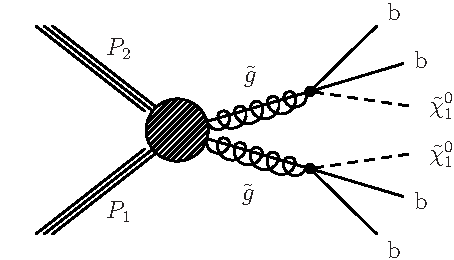
\includegraphics[width=0.3\textwidth]{figures/susyResults/T1bbbb_feyn}
    } ~~
    \subfigure[T1qqqq]{
      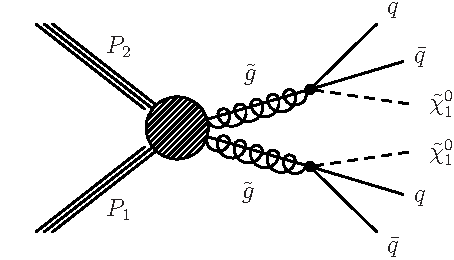
\includegraphics[width=0.3\textwidth]{figures/susyResults/T1qqqq_feyn}
    } ~~
    \subfigure[T1tttt]{
      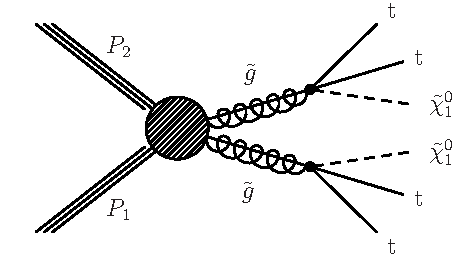
\includegraphics[width=0.3\textwidth]{figures/susyResults/T1tttt_feyn}
    } \\
    %% \subfigure[T2tt]{
    %%   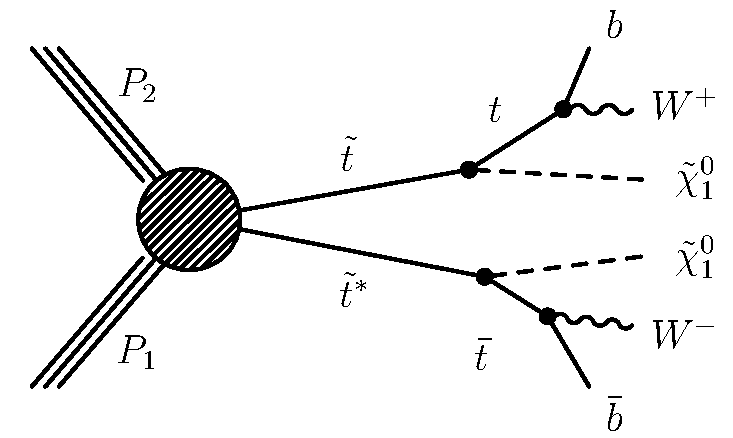
\includegraphics[width=0.3\textwidth]{figures/susyResults/T2tt_feyn}
    %% } ~~
    %% \subfigure[T2cc]{
    %%   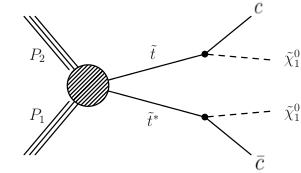
\includegraphics[width=0.3\textwidth]{figures/susyResults/T2cc_feyn.png}
    %% } ~~
    %% \subfigure[T2qq]{
    %%   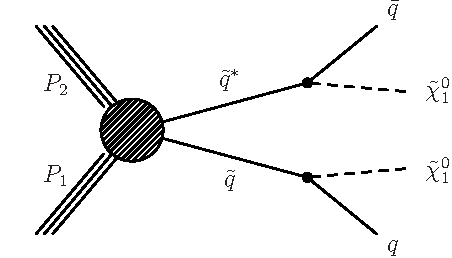
\includegraphics[width=0.3\textwidth]{figures/susyResults/T2qq_feyn}
    %% } 
    \caption{
      Graphical representation of the production and decay of supersymmetric particles in the 
      simplified models considered in the analysis. 
    }
    \label{fig:simplified-models}
  \end{center}
\end{figure}



\subsection{Signal acceptance and contamination}
\label{sec:sig-accept-contam}
The signal efficiency times acceptance for the simplified models used in the analysis 
is shown in Fig.~\ref{fig:sig-eff}. 
These efficiencies are computed including the 4 best categories used to extract the limits w(see Sec.~\ref{sec:susy_results}).

\begin{figure}[h!]
  \begin{center}
    \subfigure[T1bbbb]{
      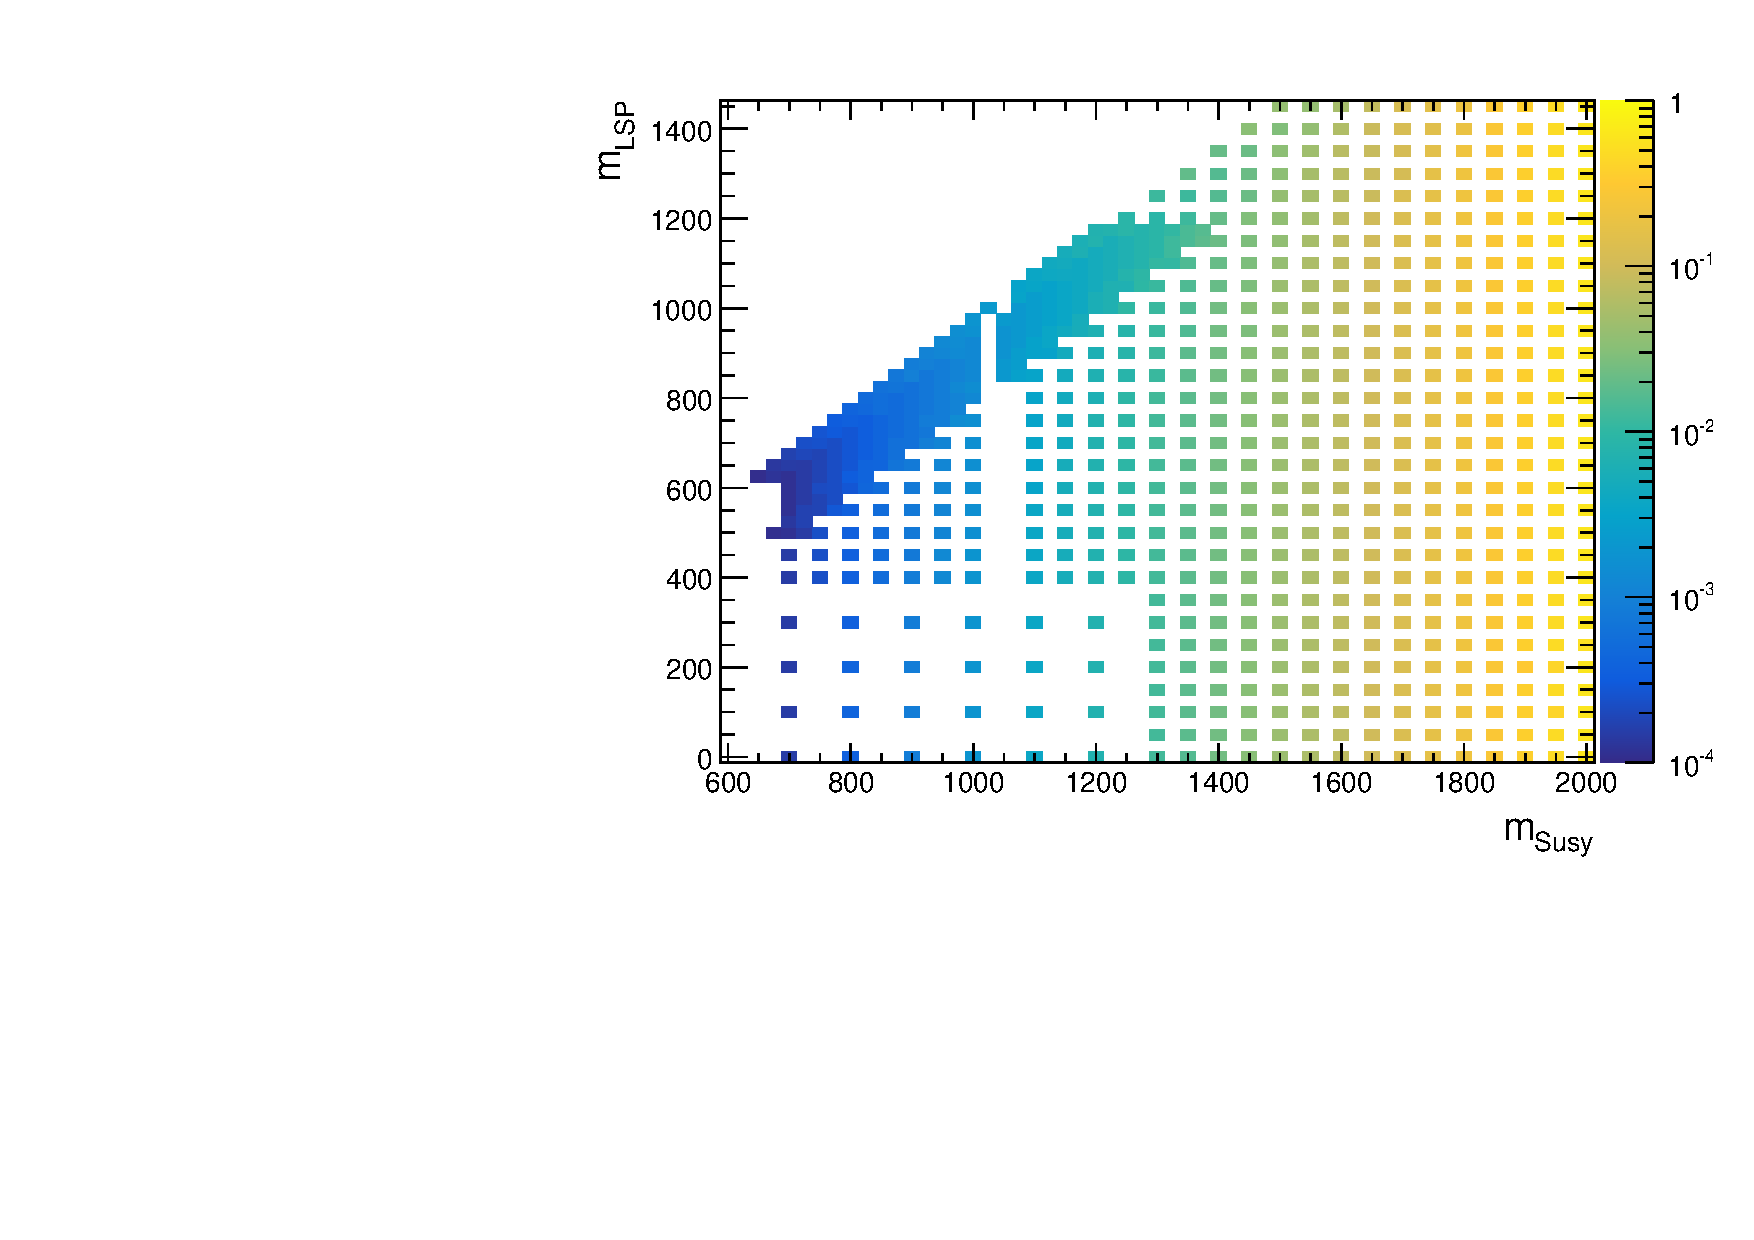
\includegraphics[width=0.5\textwidth]{figures/susyResults/T1bbbb_merging_4_cats.pdf}
    } ~~
    \subfigure[T1qqqq]{
      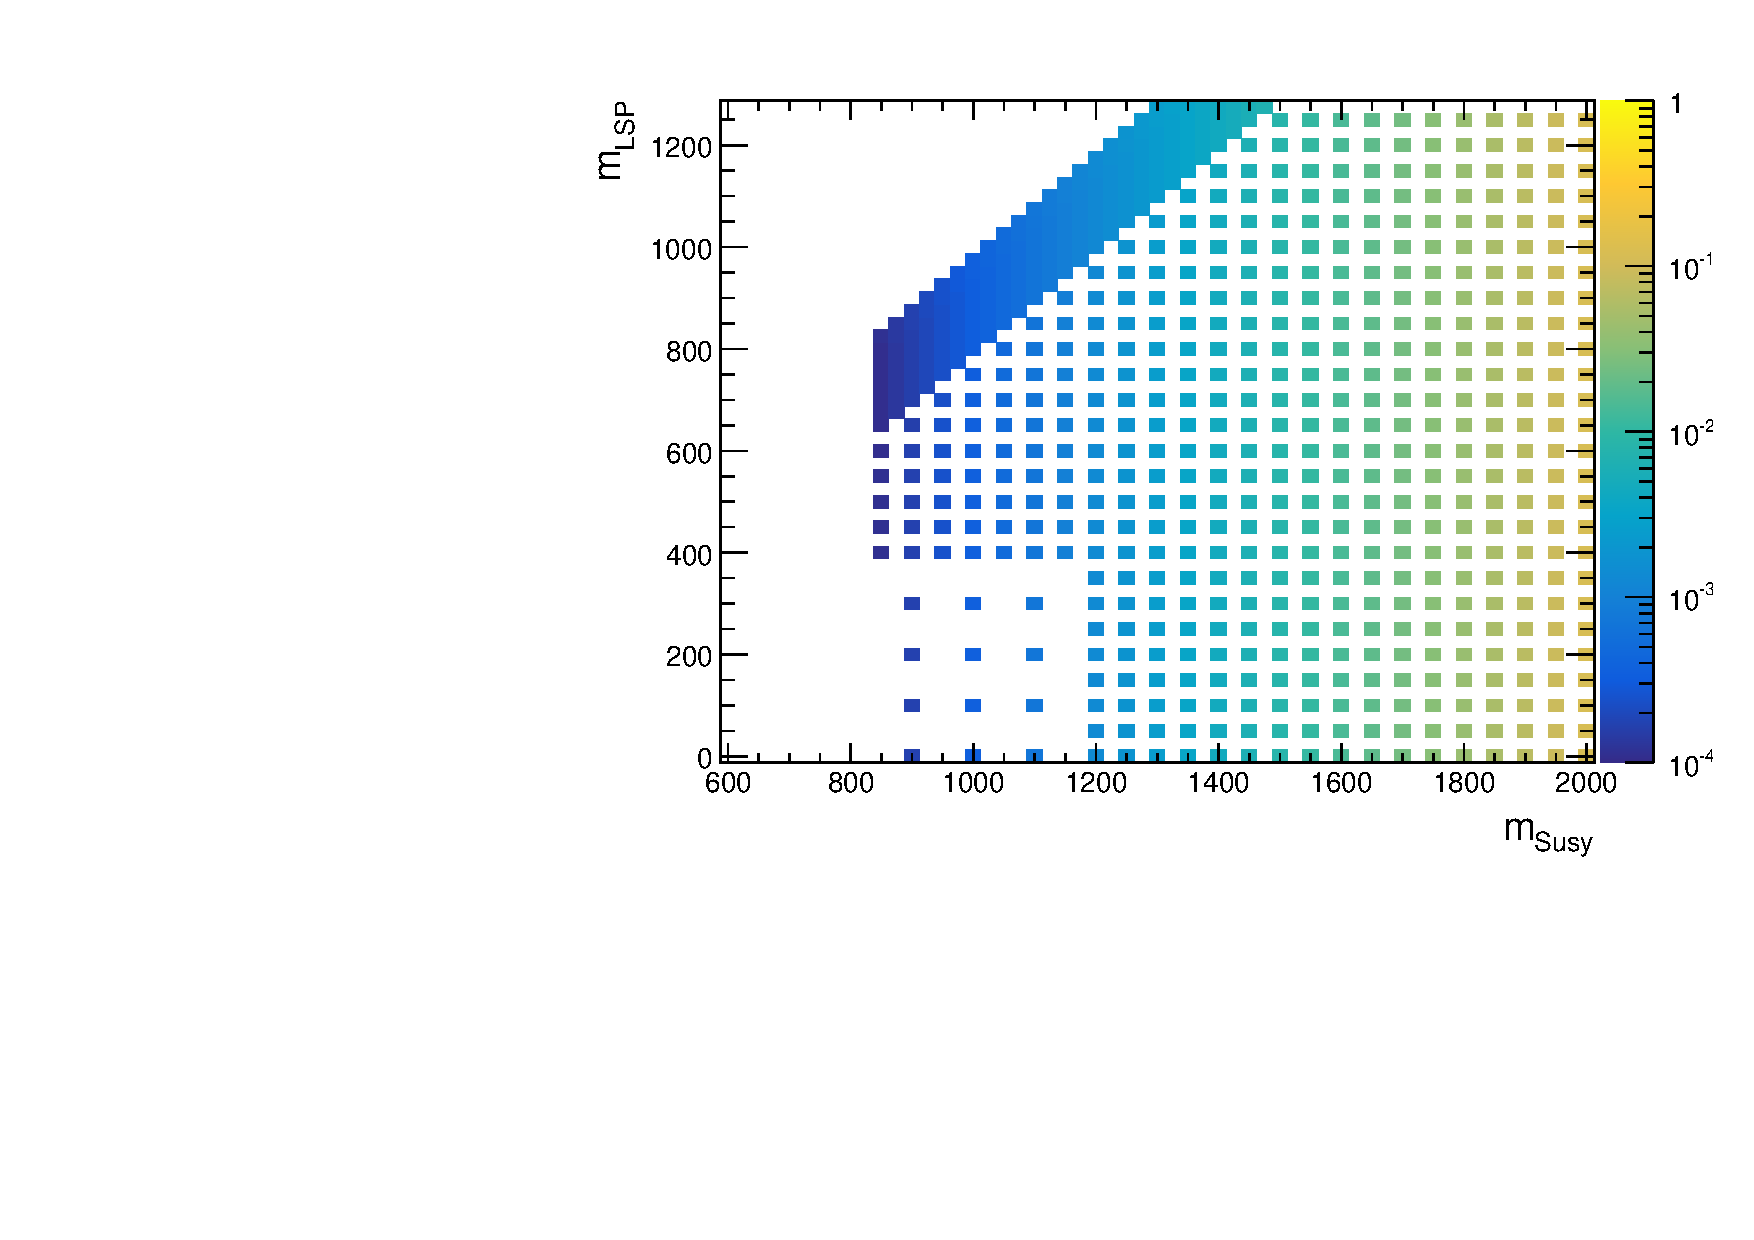
\includegraphics[width=0.5\textwidth]{figures/susyResults/T1qqqq_merging_4_cats.pdf}
    } \\
    \subfigure[T1tttt]{
      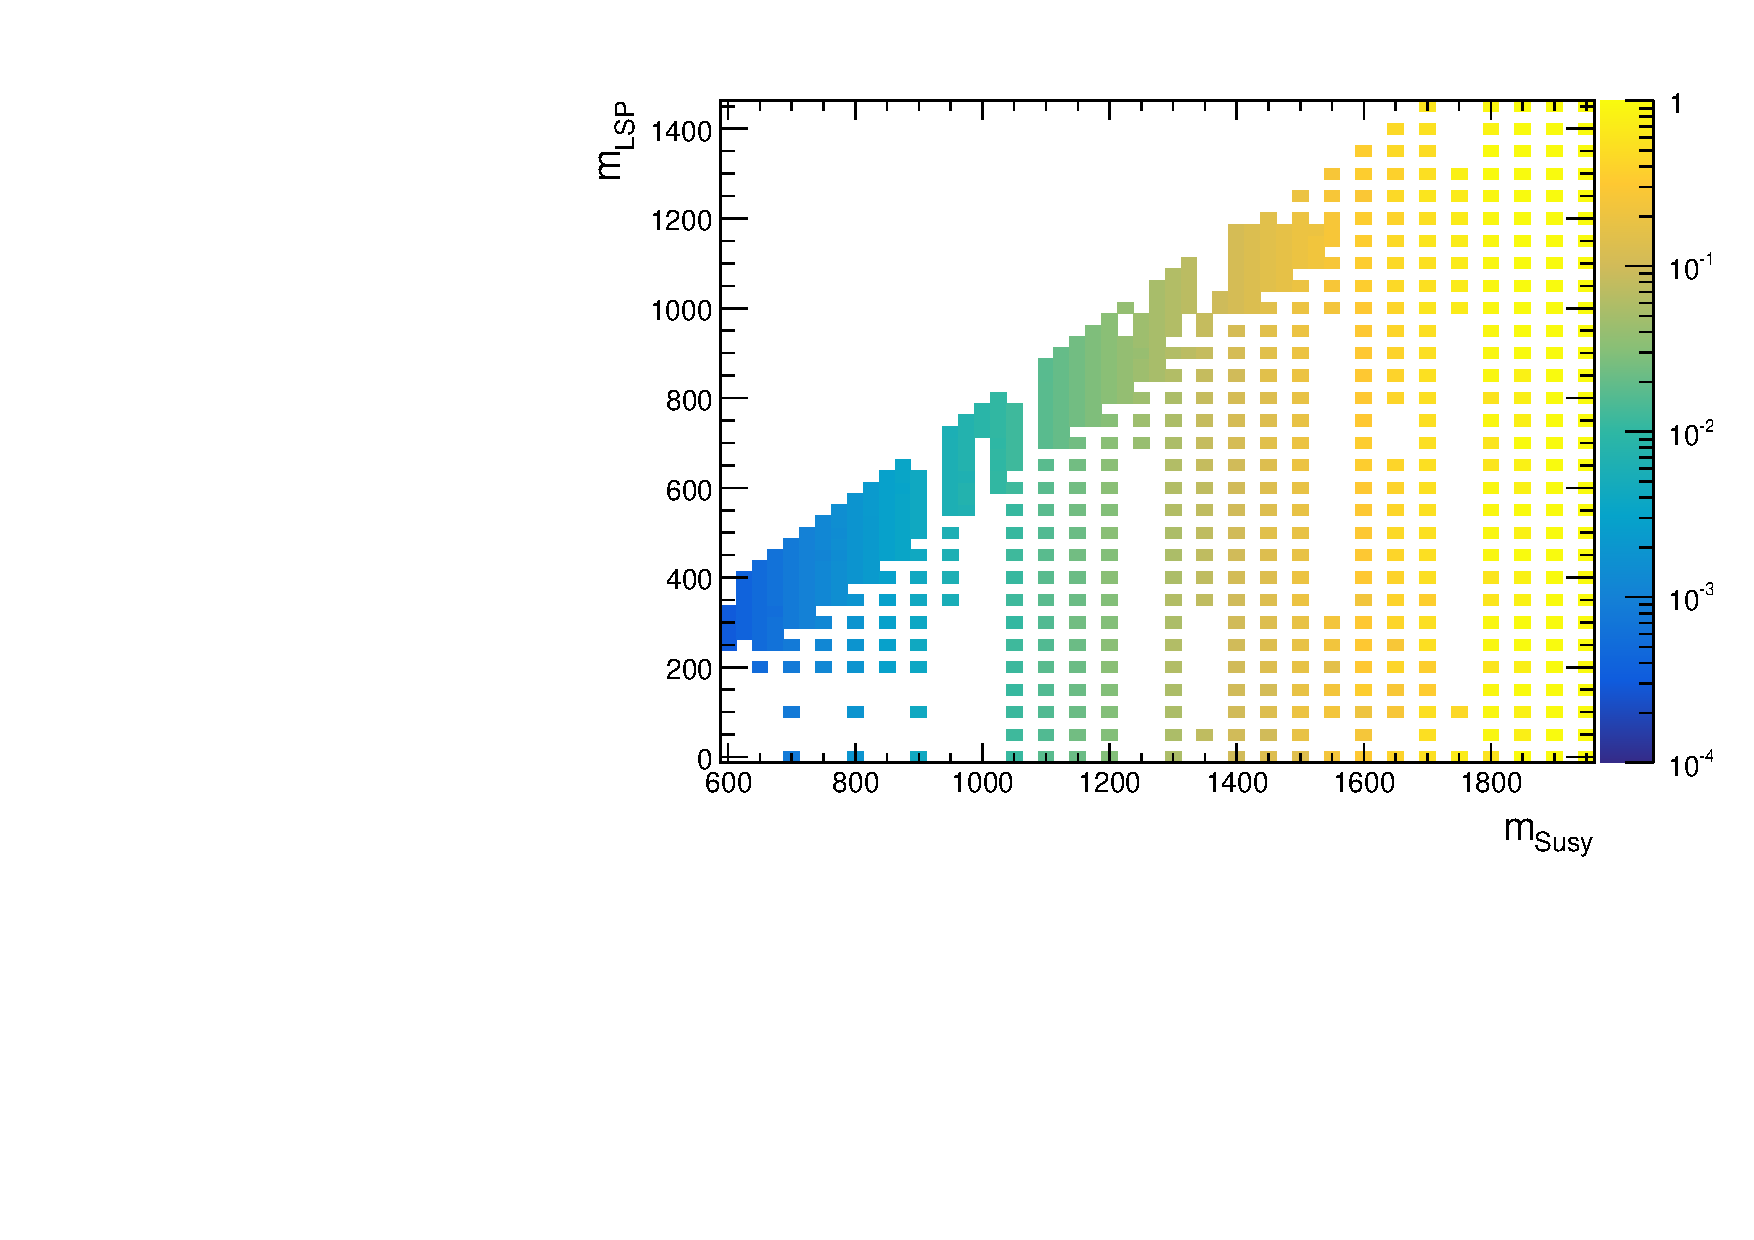
\includegraphics[width=0.5\textwidth]{figures/susyResults/T1tttt_merging_4_cats.pdf}
    } \\
    %% \subfigure[T2tt]{
    %%   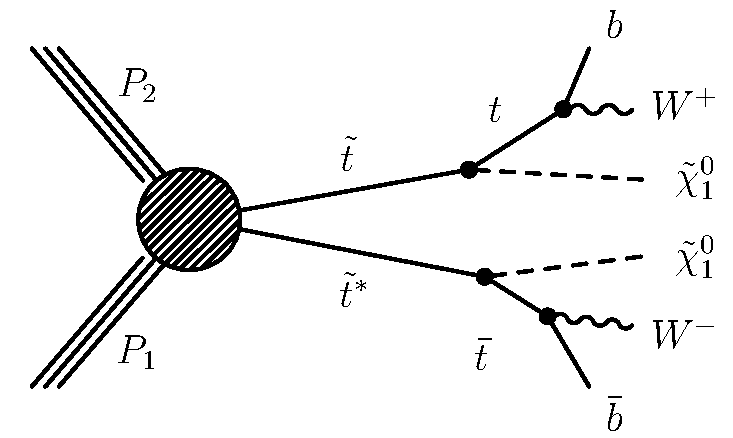
\includegraphics[width=0.3\textwidth]{figures/susyResults/T2tt_feyn}
    %% } ~~
    %% \subfigure[T2cc]{
    %%   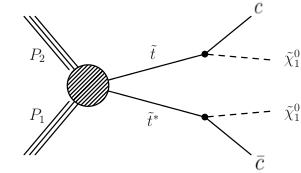
\includegraphics[width=0.3\textwidth]{figures/susyResults/T2cc_feyn.png}
    %% } ~~
    %% \subfigure[T2qq]{
    %%   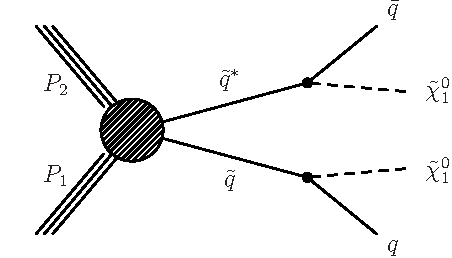
\includegraphics[width=0.3\textwidth]{figures/susyResults/T2qq_feyn}
    %% } 
    \caption{
      Efficiency times acceptance for the signal models as a function of $m_{\mathrm{Susy}}$ and $m_{\mathrm{LSP}}$.
    }
    \label{fig:sig-eff}
  \end{center}
\end{figure}

The level of signal contamination in the control regions is expected to be negligible 
for most of the models that are targeted by this search. 
The requirement of one muon, two muons or one photon in the \mj, \mmj and \gj respectively 
ensures that the control regions are depleted signal events. 
The only partial exception is the gluino pair production and stop pair production followed by decay into top quarks, 
called T1tttt and T2tt respectively. 
In this case, when top decays leptonically a residual signal contamination may be found in the muon control regions. \\

Figure~\ref{fig:contamination} characterises the level of signal
contamination in the \mj control sample for the benchmark model
T2tt ($m_{\mathrm{Stop}}=600$ GeV, $m_{\mathrm{LSP}}=100$ GeV) relative to the signal acceptance in the
signal region. Figures~\ref{fig:contamination} (a) and (b) show the
expected signal yield counts as a function of event category and
\scalht bin in the signal and \mj control regions, respectively.

\begin{figure}[h!]
  \begin{center}
    \subfigure[Expected counts in the signal region]{
      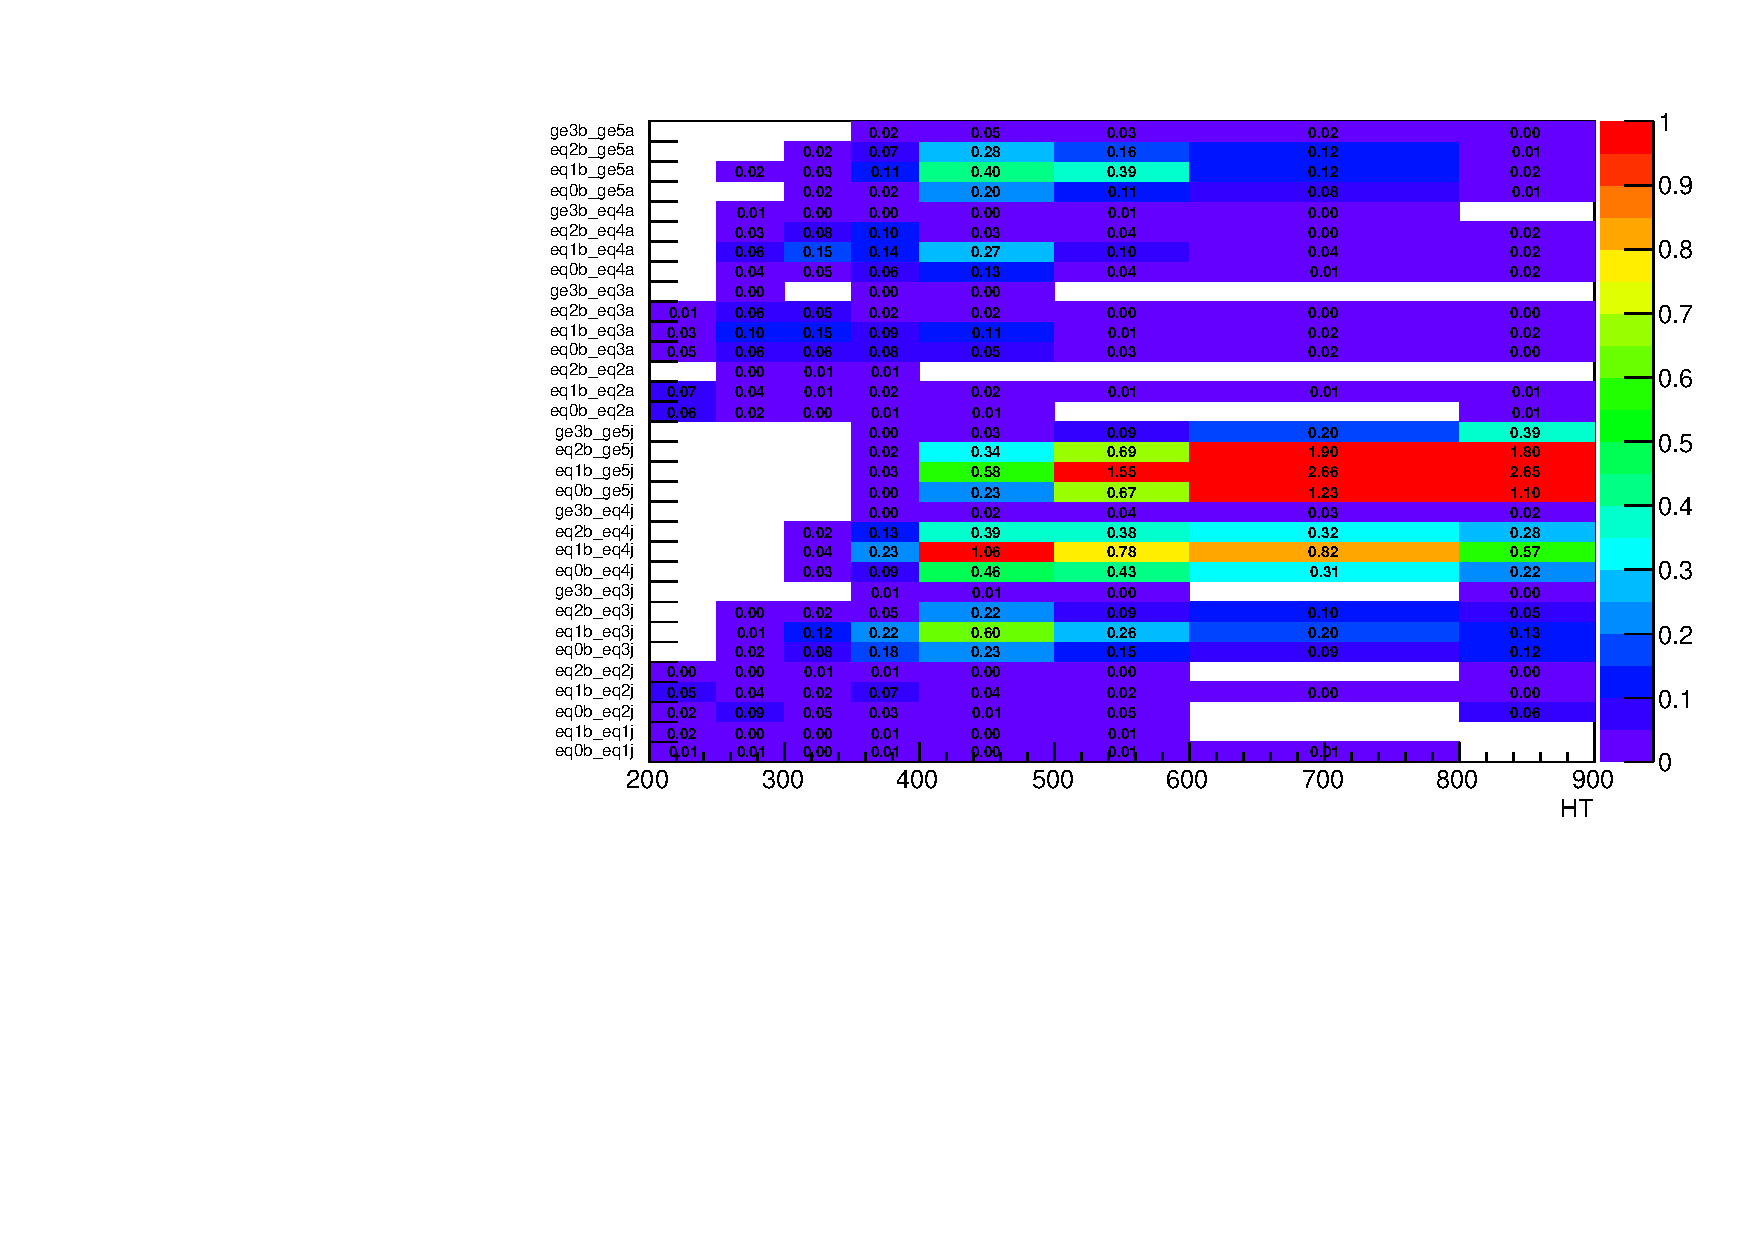
\includegraphics[width=0.5\textwidth]{figures/susyResults/sigYields_had_SMS-T2tt_mStop-600_mLSP-100_25ns}
    } 
    \subfigure[Expected counts in the \mj control region]{
      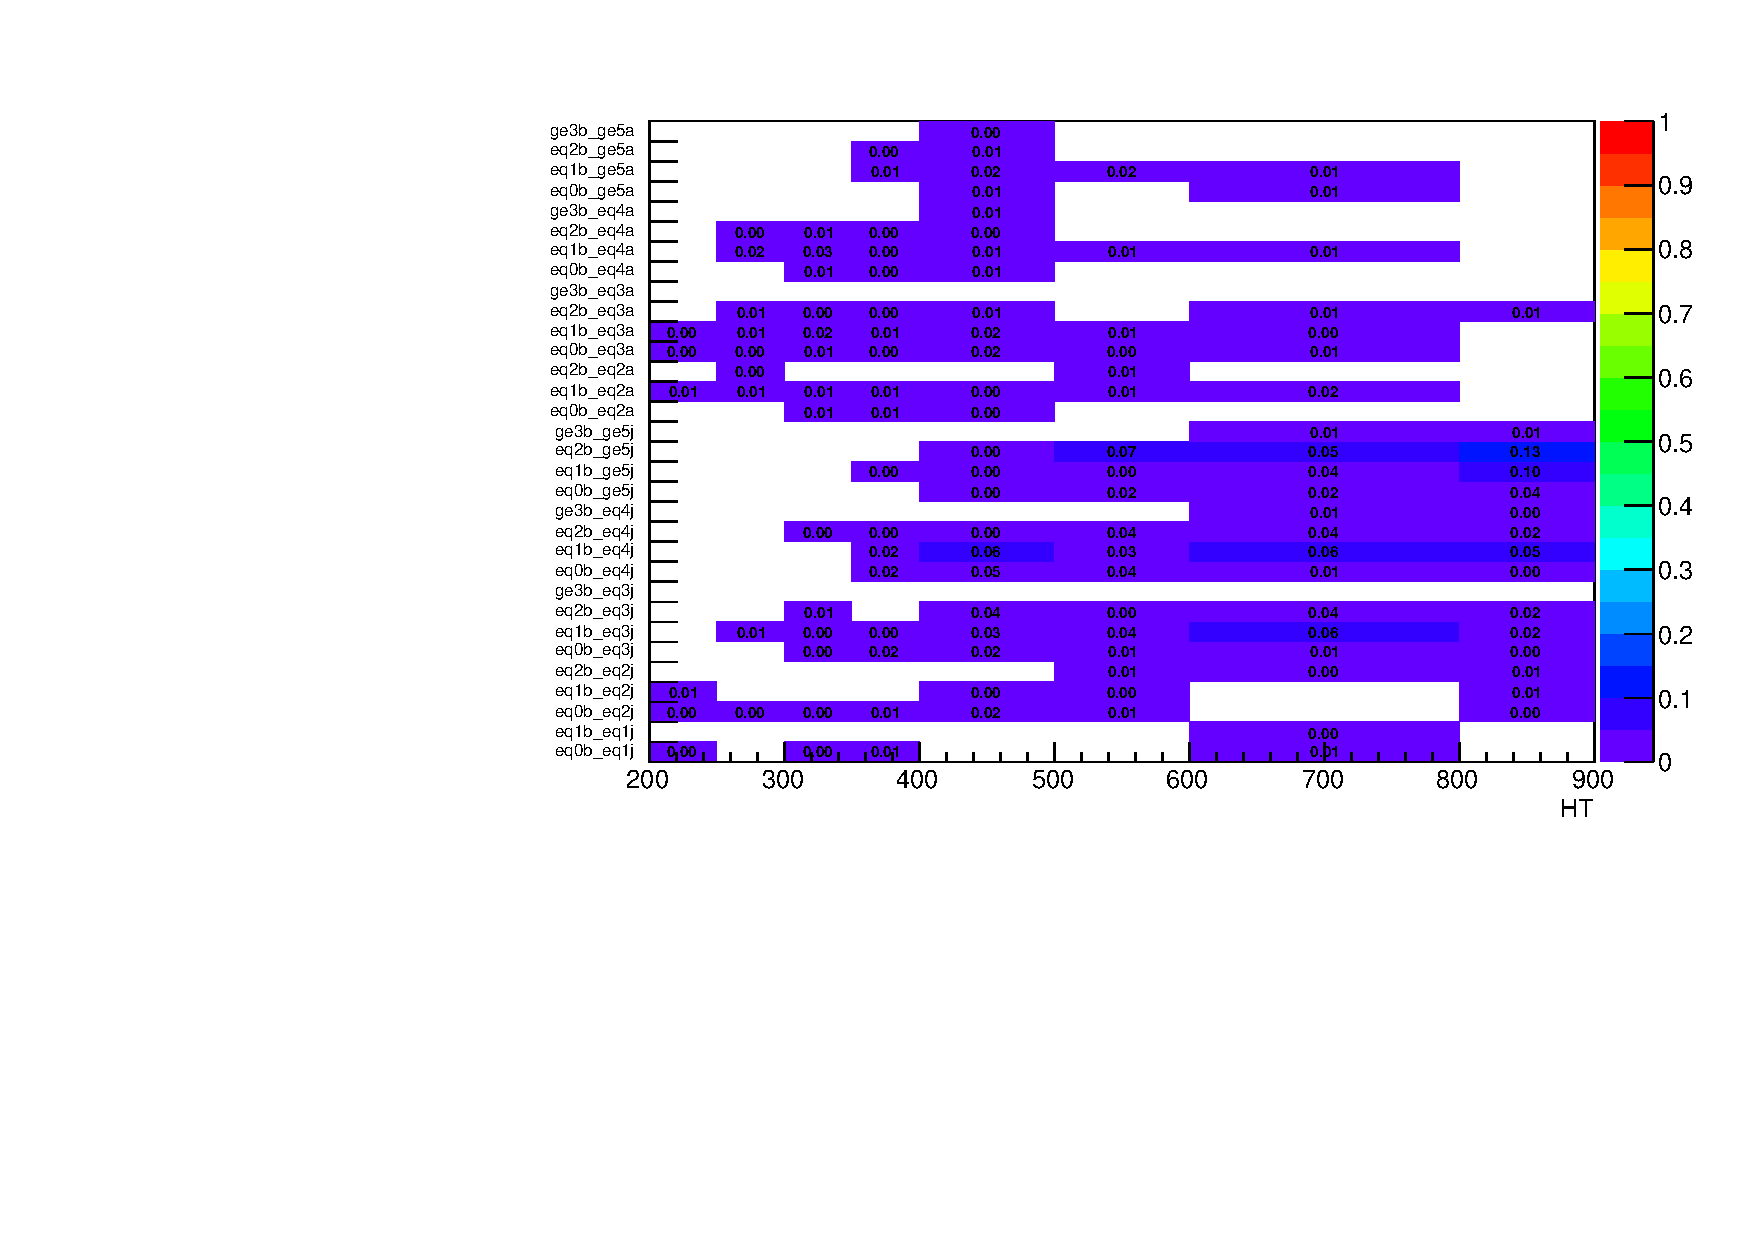
\includegraphics[width=0.5\textwidth]{figures/susyResults/sigYields_SingleMu_SMS-T2tt_mStop-600_mLSP-100_25ns}
    } \\
    \subfigure[Ratio of signal acceptance (\mj control region divided by signal region)]{
      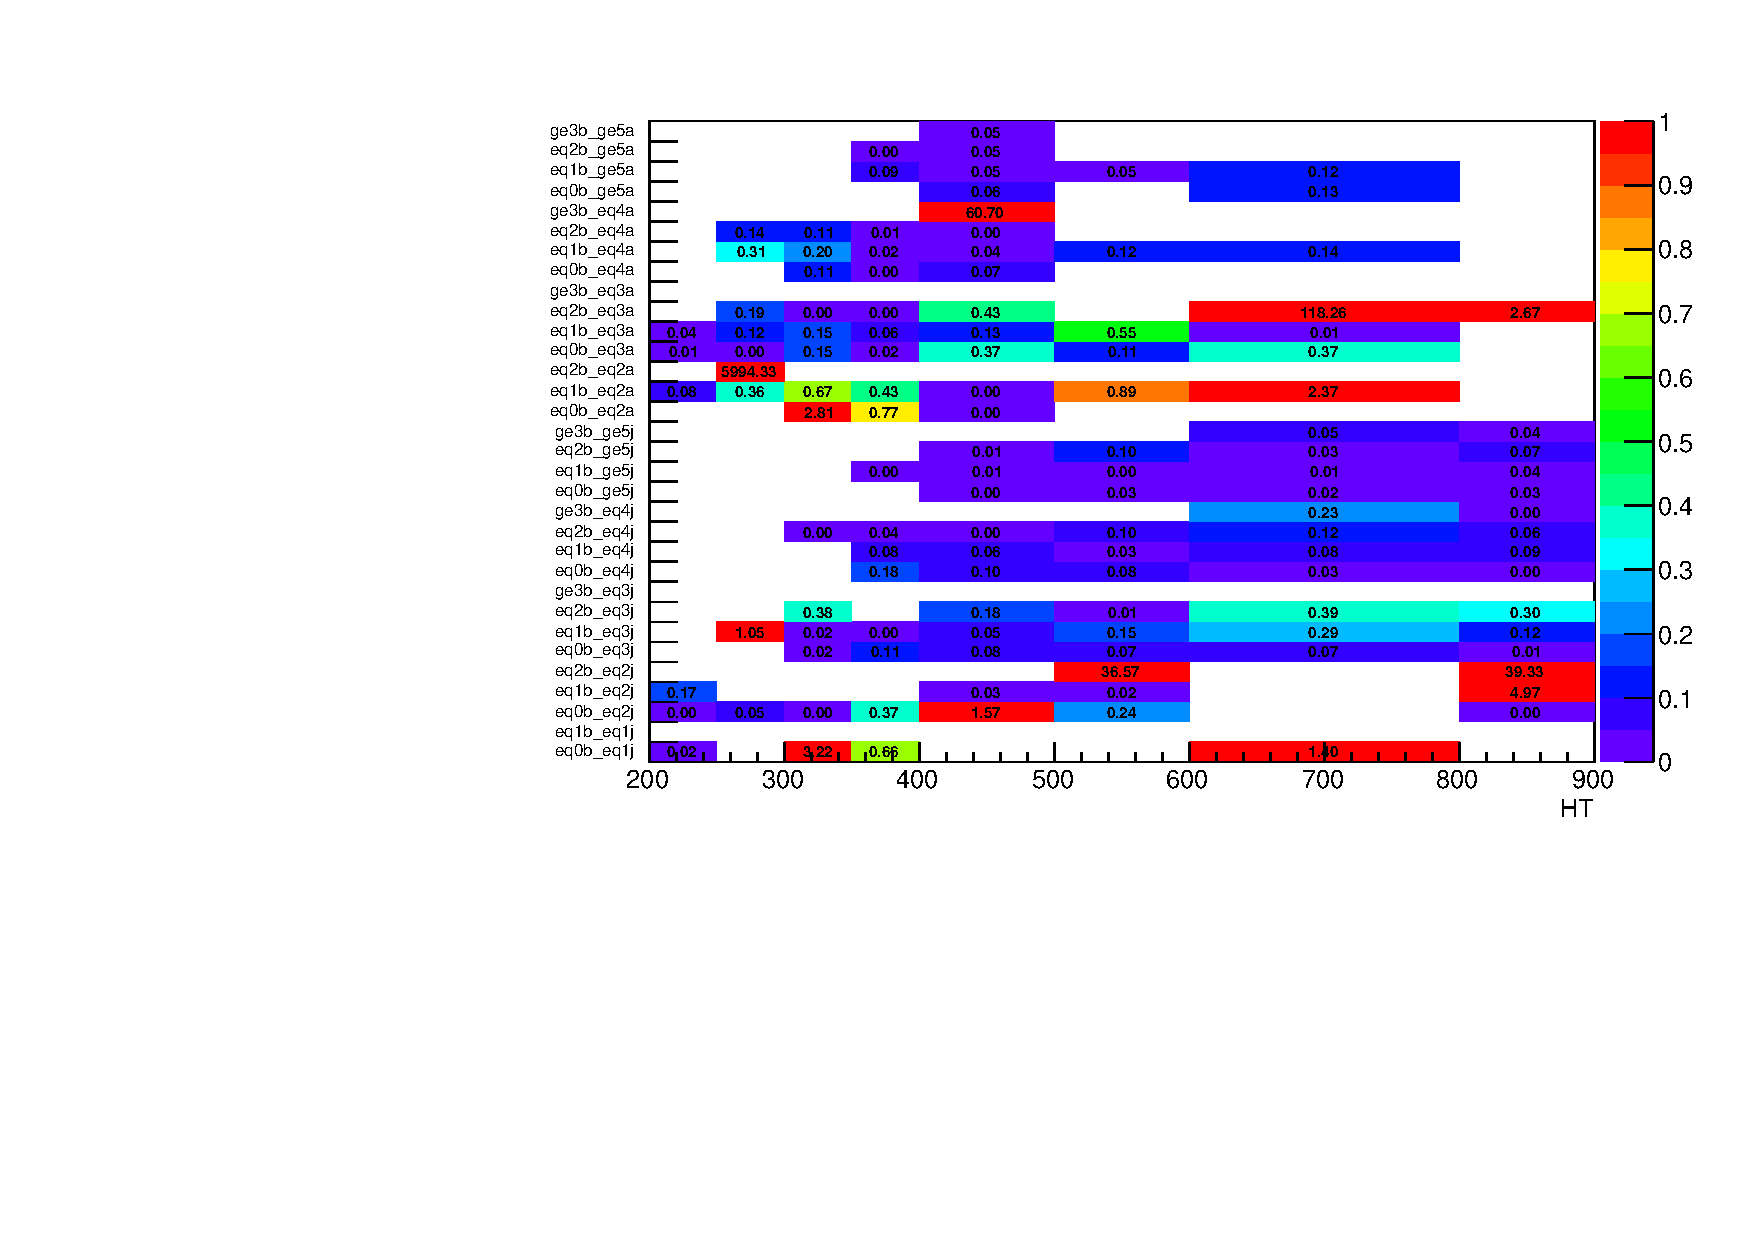
\includegraphics[width=0.5\textwidth]{figures/susyResults/relEff_SingleMu_SMS-T2tt_mStop-600_mLSP-100_25ns}
    }
    \subfigure[Ratio of S/B values (signal region w.r.t. \mj)]{
      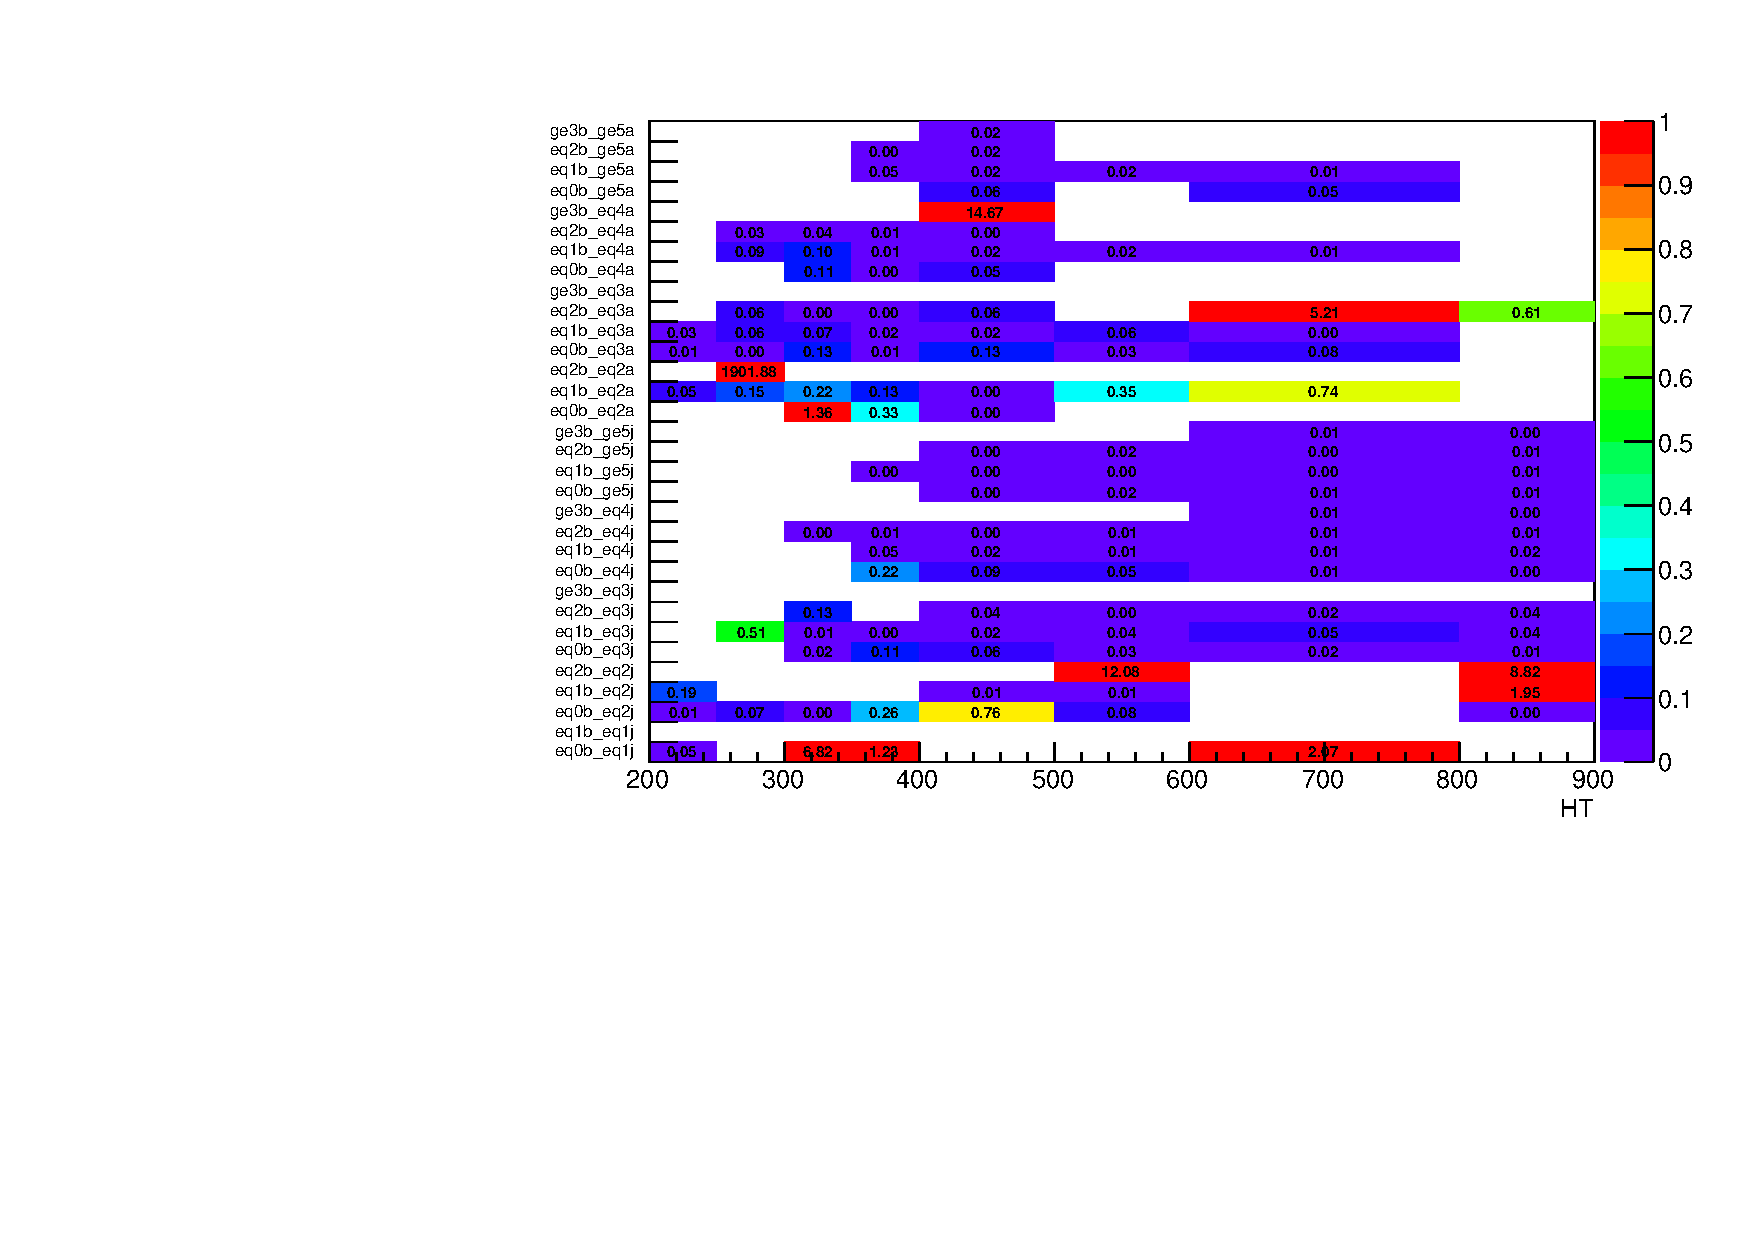
\includegraphics[width=0.5\textwidth]{figures/susyResults/doubleRatio_SingleMu_SMS-T2tt_mStop-600_mLSP-100_25ns}
    }
    \caption{Characterisation of signal acceptance and contamination
      in the signal and \mj control regions, respectively, for the
      benchmark model T2tt (600,100).}
    \label{fig:contamination}
  \end{center}
\end{figure}

Figure~\ref{fig:contamination} (c) shows the ratio of these expected
yields (signal region with respect to the \mj control region). The
ratio is typically small, at the percent level for the most sensitive
categories (\ie with four or more jets and one or two b-tagged jets).

In addition, the event counts from SM background processes in the \mj
control sample are significantly higher than in the signal region, as
no \alphat requirement is made for the \mj sample. Therefore, the S/B
ratios for the signal region relative to the \mj sample are larger by
many factors, typically $\gg$10. Figure~\ref{fig:contamination} (d)
shows the ratio of S/B$_{\rm signal}$ over S/B$_{\rm \mj}$ as a
function of the event category and \scalht bin.

Figure~\ref{fig:contamination_t1tttt} characterises the level of
signal contamination in the \mj control sample for the benchmark model
T1tttt ($m_{\mathrm{Gluino}}=1400$ GeV, $m_{\mathrm{LSP}}=100$ GeV). A larger level of contamination is
expected for this model (with respect to T2tt), due to the
presence of four W bosons produced in the decay of the gluino-pair
system (via off-shell top squarks). The ratio of yields in the signal
and \mj control regions is at the level of $\sim$10--20\% for the most
sensitive categories (\ie with four or more jets, two or more b-tagged
jets, and at high \scalht). The ratio of S/B values for the signal
region relative to the \mj sample is still large, typically $\gg$10.

\begin{figure}[h!]
  \begin{center}
    \subfigure[Expected counts in the signal region]{
      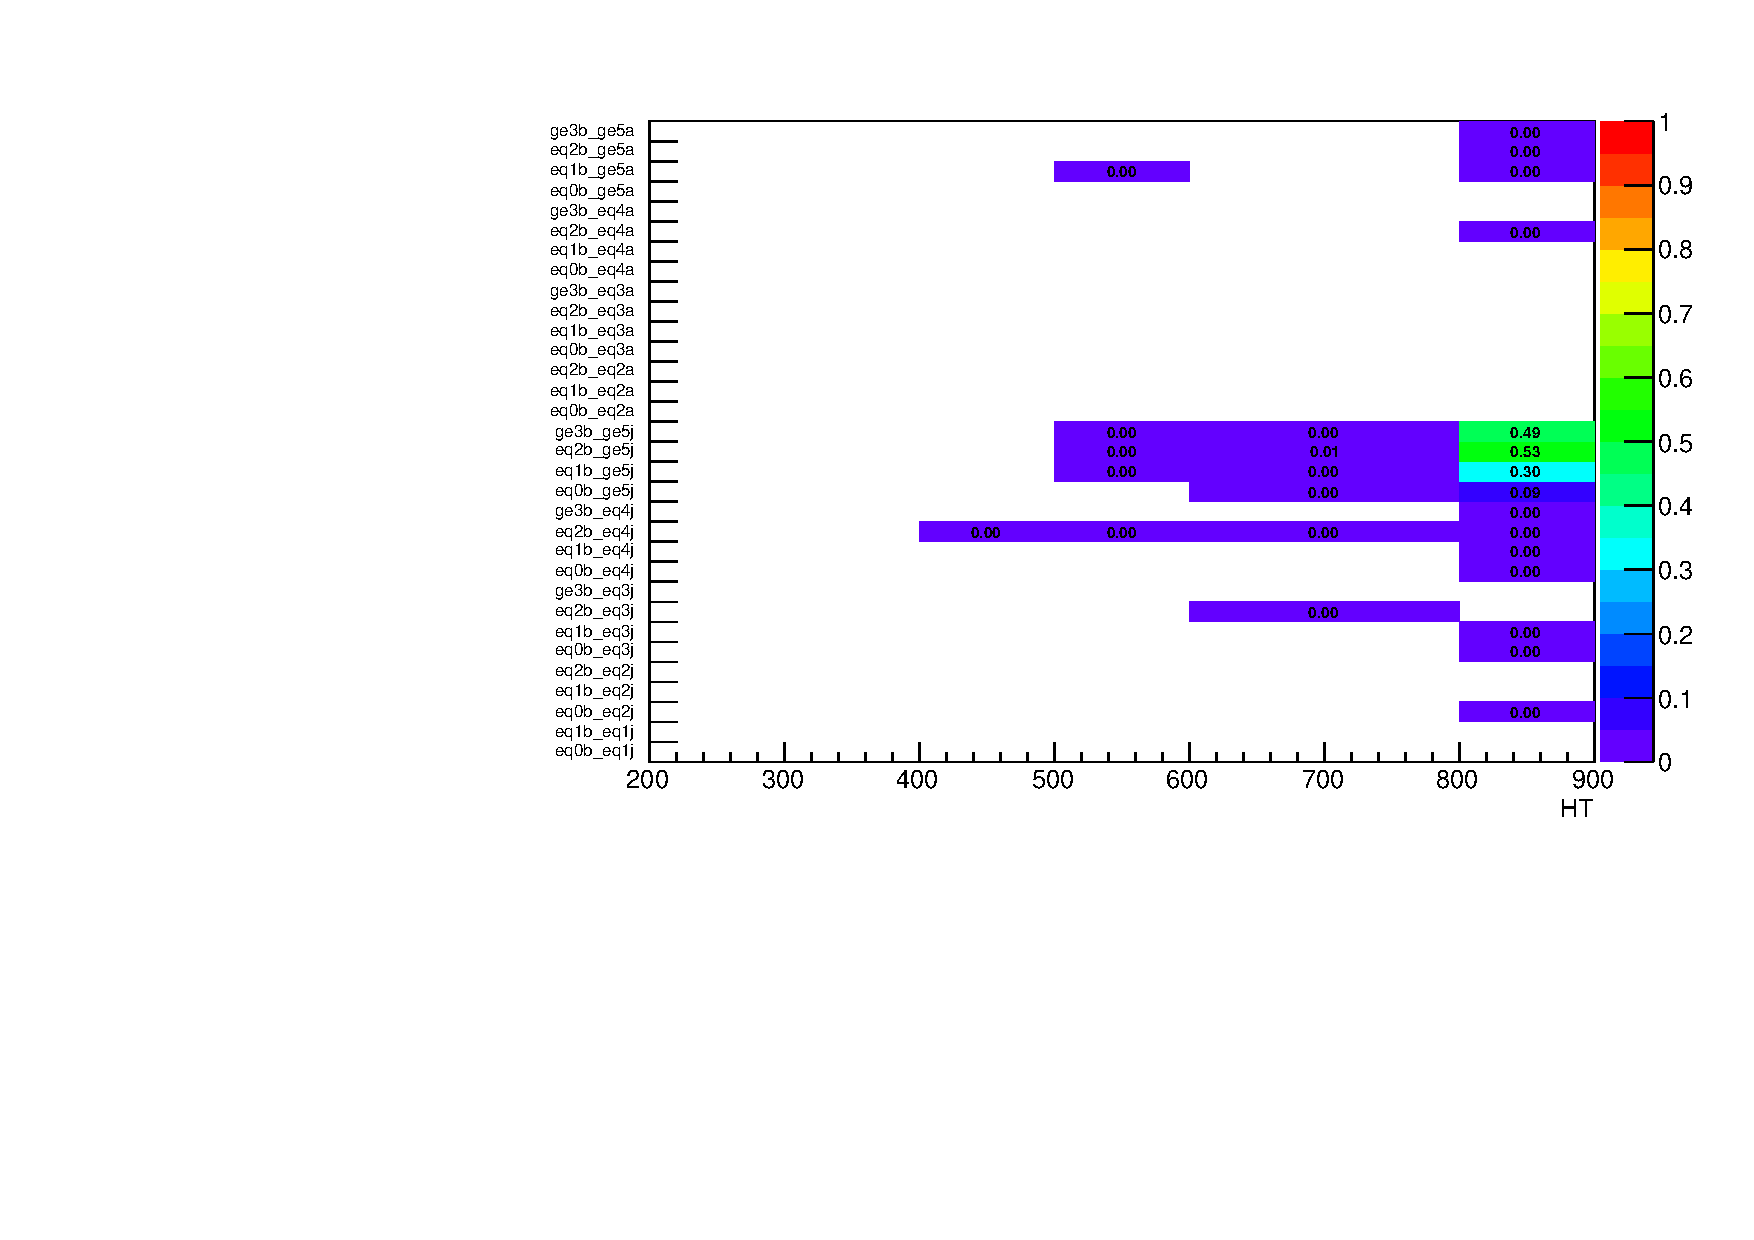
\includegraphics[width=0.5\textwidth]{figures/susyResults/sigYields_had_SMS-T1tttt_mGluino-1400_mLSP-100_25ns}
    } 
    \subfigure[Expected counts in the \mj control region]{
      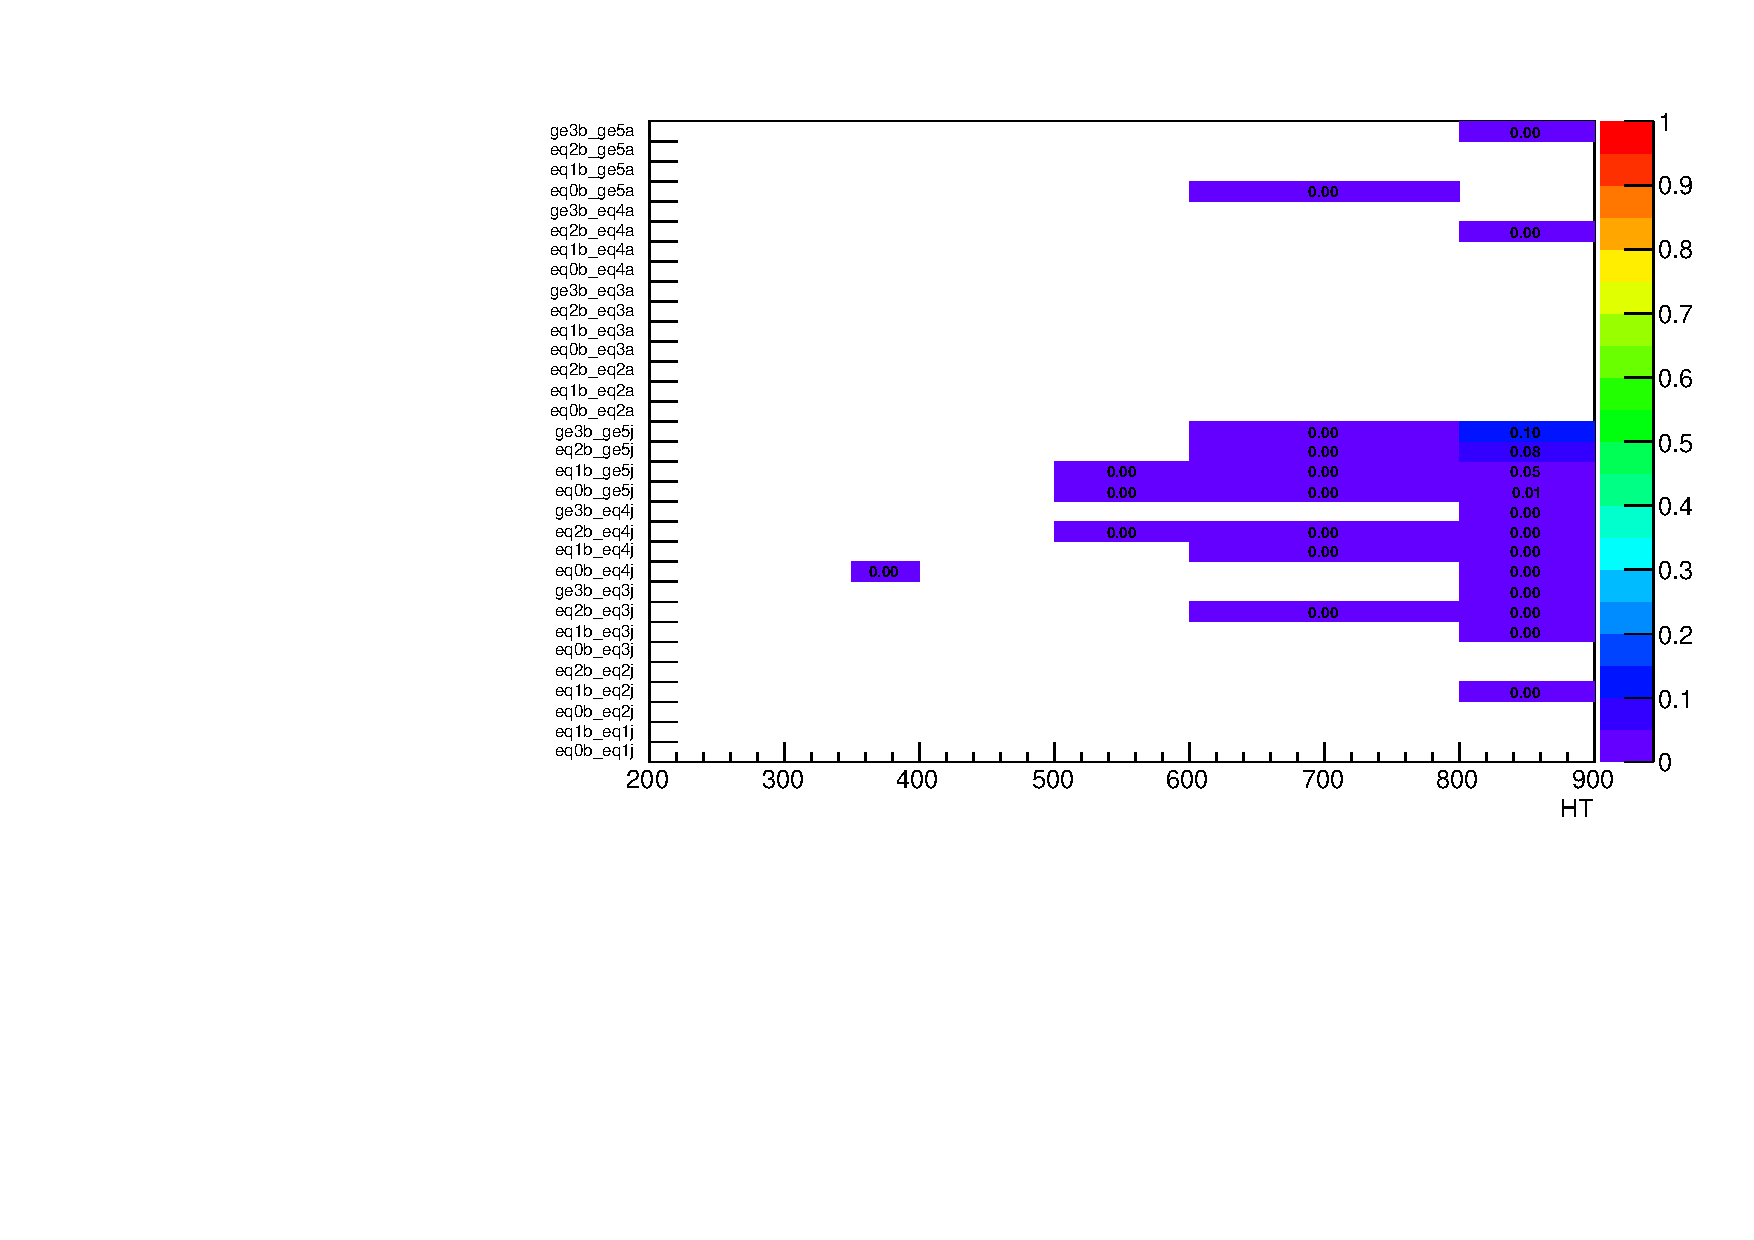
\includegraphics[width=0.5\textwidth]{figures/susyResults/sigYields_SingleMu_SMS-T1tttt_mGluino-1400_mLSP-100_25ns}
    } \\
    \subfigure[Ratio of signal acceptance (\mj control region divided by signal region)]{
      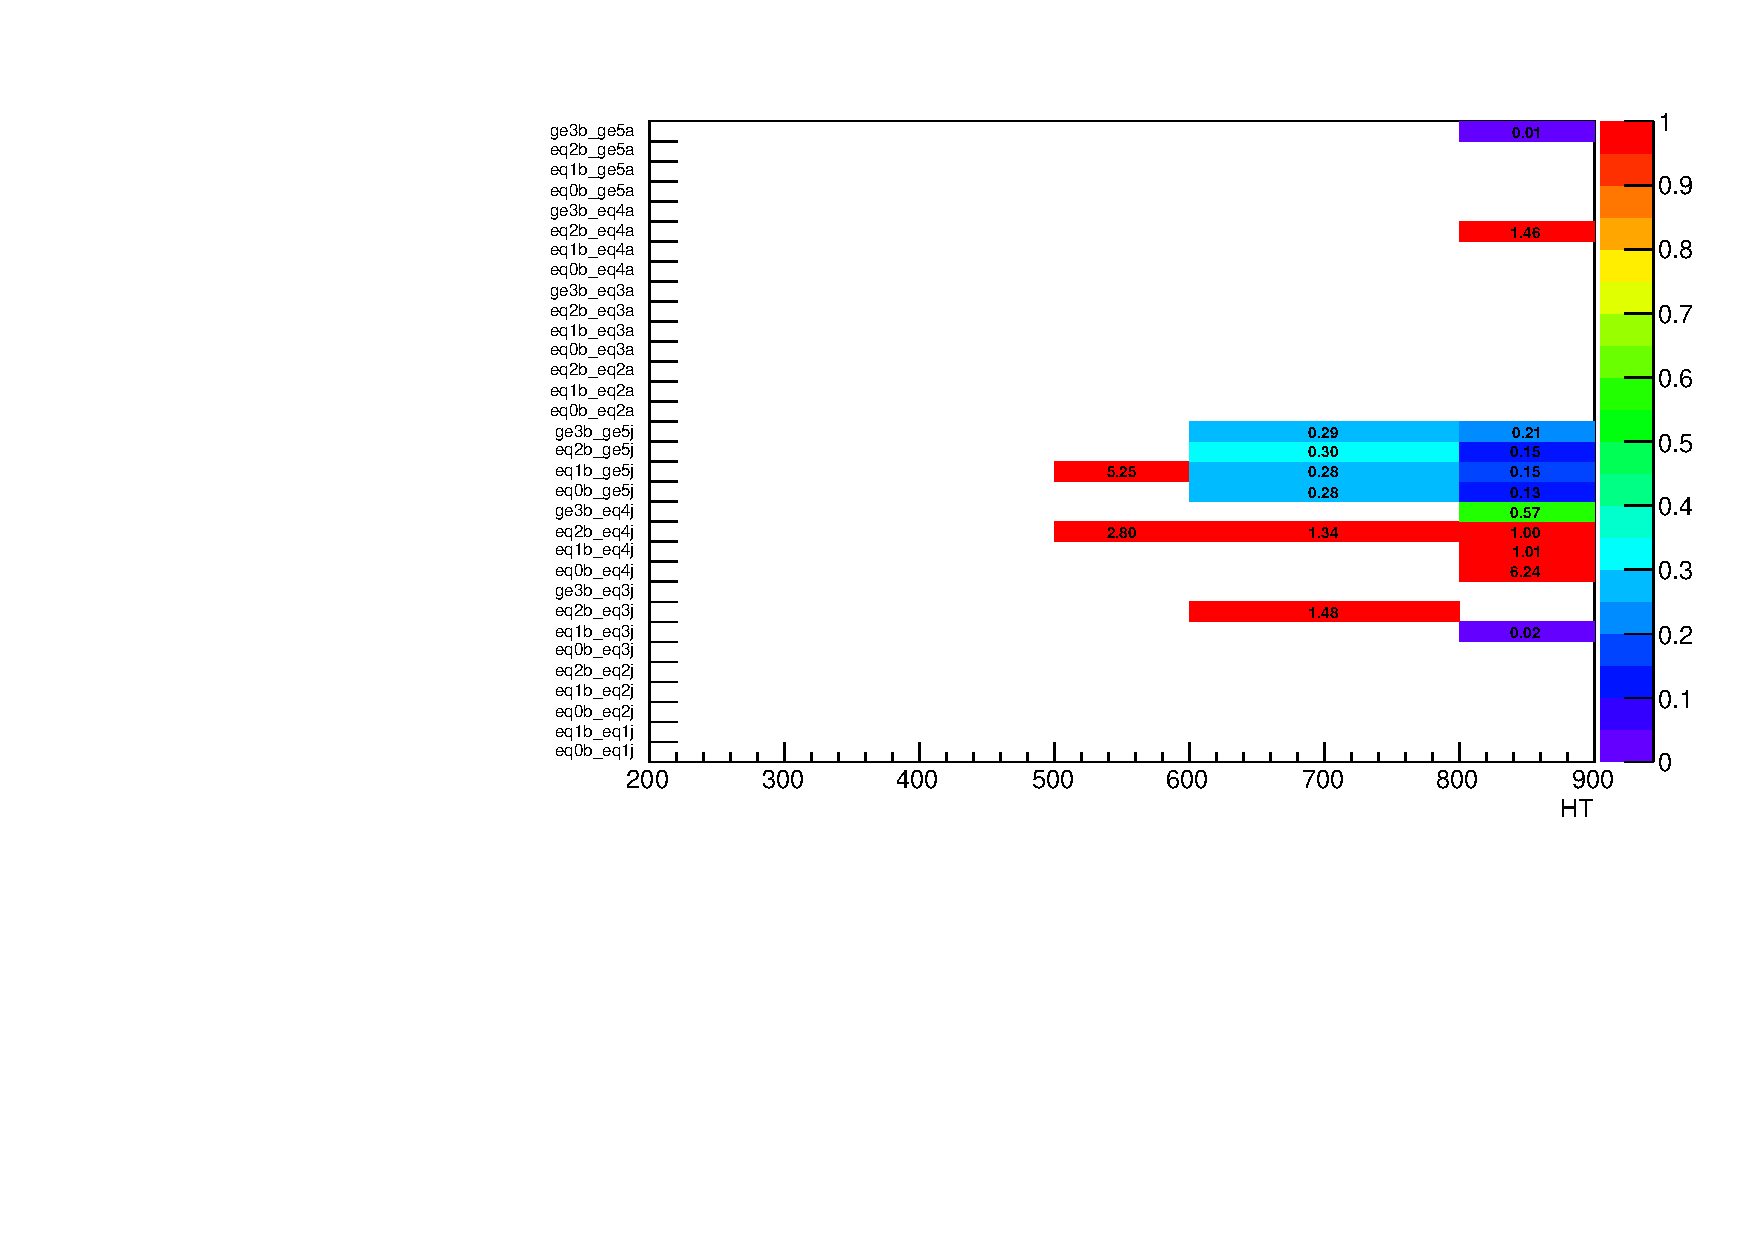
\includegraphics[width=0.5\textwidth]{figures/susyResults/relEff_SingleMu_SMS-T1tttt_mGluino-1400_mLSP-100_25ns}
    }
    \subfigure[Ratio of S/B values (signal region w.r.t. \mj)]{
      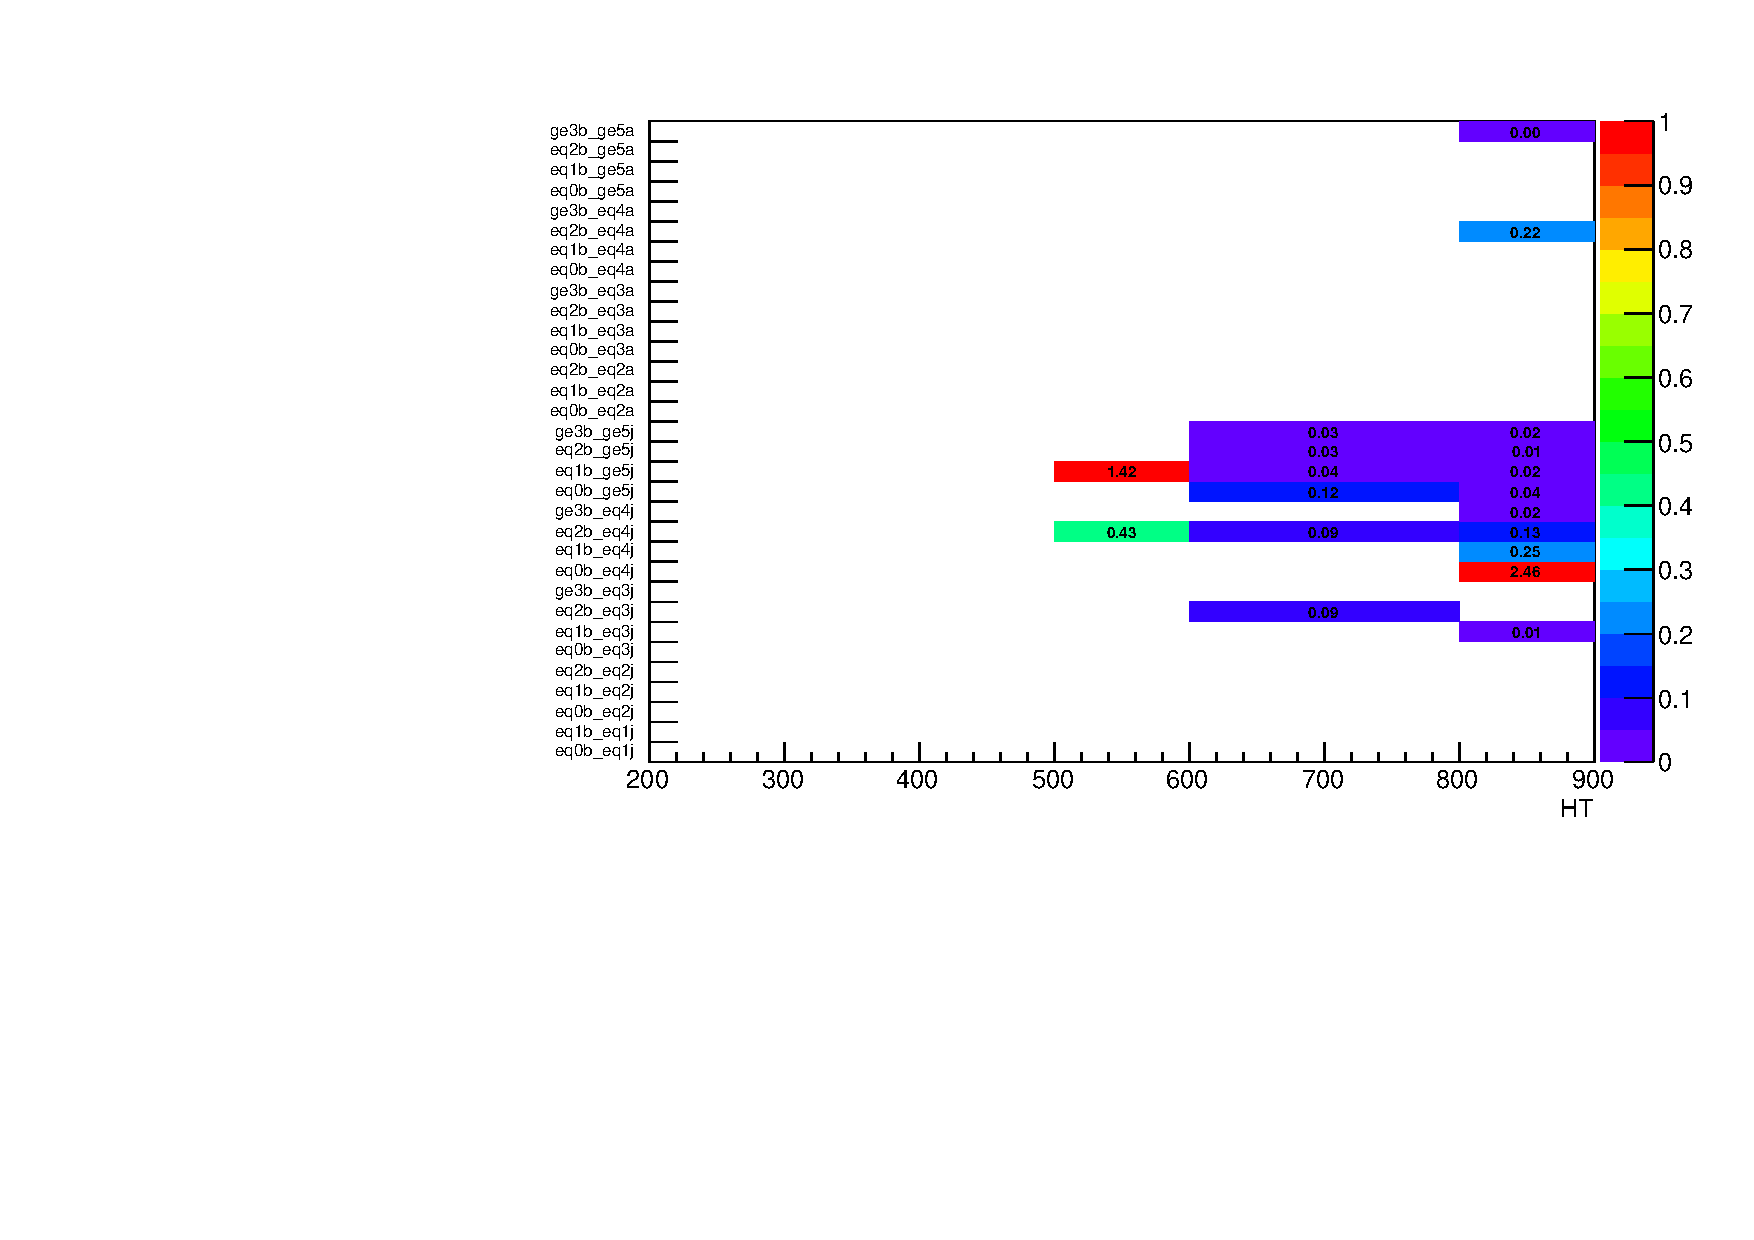
\includegraphics[width=0.5\textwidth]{figures/susyResults/doubleRatio_SingleMu_SMS-T1tttt_mGluino-1400_mLSP-100_25ns}
    }
    \caption{Characterisation of signal acceptance and contamination
      in the signal and \mj control regions, respectively, for the
      benchmark model T1tttt (1400,100).}
    \label{fig:contamination_t1tttt}
  \end{center}
\end{figure}

For both models the level of contamination for the
\mmj sample is smaller still due to the requirement of a second
muon. The contamination for the \gj sample is expected to be zero for
the models under consideration. 

Finally, the potential for signal contamination in all control samples
is fully accounted for in the likelihood model used to extract
information on sensitivity to any given signal model.

\subsection{Systematic uncertainties on signal efficiency times acceptance}
\label{sec:sig-syst}
The following sources of systematic uncertainty are propagated to the signal acceptance and shape, 
according to the recommendations agreed on within the collaboration. 
Relative effect on the yields are presented in Tab.~\ref{tab:sig-systematics} for some benchmark models. 

\begin{itemize}
  \item Luminosity: 4.6 \%, taken as correlated across all bins.
  \item Trigger: conservatively, the size of the inefficiency is taken as systematic variation 
    where not in the plateau (see Sec.~\ref{sec:triggers}). 
  \item MC statistics:  uncorrelated bin-by-bin uncertainty, affecting the shape of the signal. 
  \item Pileup reweighting: 5\% uncertainty on the minimum bias cross section (see Sec.~\ref{sec:pileup-reweighting}).
  \item b-tag efficiency: uncertainty on the FullSim and FastSim b-tag scale factor is propagated and taken as correlated across the bins. 
  \item Lepton efficiency: uncertainty on the lepton scale factors is propagated and taken as correlated across the bins. 
  \item Jet energy scale: uncertainty on the jet energy corrections is propagated and taken as correlated across the bins.
  \item Initial State Radiation (ISR): 15\% (30\%) uncertainty for the \Pt of the gluino-gluino system between 400-600 GeV (above 600 GeV). 
\end{itemize}


\begin{table}[h!]
  \caption{Representative range of uncertainty across the analysis bins 
    for each source of signal systematic.
    Two benchmark point are chosen for each model, 
    corresponding to ``compressed'' and ``uncompressed'' scenarios, 
    i.e. with small and large mass splitting between the mother particle and the LSP.
  }
  \label{tab:sig-systematics}
  \centering
  \begin{tabular}{ ccccc }
    \hline
    \hline
    Systematic & \multicolumn{2}{c}{T1bbbb} & \multicolumn{2}{c}{T1qqqq} & \multicolumn{2}{c}{T1tttt}  \\ 
                      & (1000,800) & (1500,100) & (900,700) & (1350,100) & (800,400) & (1300,100) \\
    \hline
    Luminosity        & 4.6\%      & 4.6\%      & 4.6\%     & 4.6\%   & 4.6\%      & 4.6\%     \\ \hline
    Trigger           & 0-15\%     & 3-5\%      & 0-15\%    & 3-5\%   & 0-15\%     & 3-5\%     \\ \hline
    MC statistics     & 0-50\%     & 0-50\%     & 0-50\%    & 0-50\%  & 0-50\%     & 0-50\%    \\ \hline
    PU reweighting    & 1-5\%      & 1-5\%      & 1-5\%     & 1-5\%   & 1-5\%      & 1-5\%     \\ \hline
    B-tag efficiency  & 0-10\%     & 0-20\%     & 0-10\%    & 0-10\%  & 0-30\%     & 0-15\%    \\ \hline
    Lepton efficiency & 10\%       & 10\%       & 10\%      & 10\%    & 10\%       & 10\%      \\ \hline
    Jet energy scale  & 5-20\%     & 0-10\%     & 5-20\%    & 0-10\%  & 0-20\%     & 0-20\%    \\ \hline
    ISR               & 0-15\%     & 1-2\%      & 0-15\%    & 1-2\%   & 0-8\%     & 1-5\%     \\
    \hline
    \hline
  \end{tabular}
\end{table}



\subsection{Exclusion limits}
\label{sec:susy_results}

In order to extract the signal contribution in the fit, the distribution of events according to the \mht variable, 
encoded as template histograms, is used as described in Sec.~\ref{sec:had-shape} and \ref{sec:likelihood}. \\
Upper limits on the cross section are computed using the $\text{CL}_{s}$ criterion \cite{CLsTechnique}. 
Asymptotic formulae \cite{AsymptoticFormulae} are utilised to approximate the distribution of the test statistics. \\
All the statistical results are produced using the \textit{combine} tool, 
provided within the HiggsAnalysis-CombinedLimit package \cite{Combine}. 

Due to CPU constraints, only 4 out of 9 jet categories (but all \nb/\scalht bins
within each category) are considered to extract the final result. 
To choose the 4 jet multiplicity categories that are combined, a raking procedure 
is used based on the expected significance. 
In Tab.~\ref{tab:sig-bestCats} the 4 jet categories used for the limits are shown for few benchmark models. 

\begin{table}[h!]
  \caption{
    The 4 best jet categories, used in the combination providing the exclusion limits, 
    for some benchmark compressed and uncompressed models used in the analysis.
  }
  \label{tab:sig-bestCats}
  \centering
  \begin{tabular}{ lll }
    \hline
    \hline
    Model & $(m_{\mathrm{Susy}},m_{\mathrm{LSP}})$ & Best categories \\ 
    \hline
    T1bbbb & (1000,800) & $\geq5j,4j,\geq5a,4a$ \\
    T1bbbb & (1500,100) & $\geq5j,4j,3j,2j$ \\
    T1qqqq & (900,700)  & $\geq5j,4j,\geq5a,4a$ \\
    T1qqqq & (1350,100)  & $\geq5j,4j,3j,2j$ \\
    T1tttt & (800,400) & $\geq5j,\geq5a,4j,4a$ \\
    T1tttt & (1350,100) & $\geq5j,\geq5a,4j,3j$ \\
    \hline
    \hline
  \end{tabular}
\end{table}

In Figure ~\ref{fig:plane_xs} the 95\% C.L. upper limits on the cross section are shown 
in the $(m_{\mathrm{Susy}},m_{\mathrm{LSP}})$ plane for the models considered in this interpretation. 
These results correspond to 2.2 \ifb of integrated luminosity. 
The exclusion contour is also shown together with $\pm1\sigma$ uncertainty. 
The band around the expected exclusion reflects the experimental uncertainty, 
while the band around the observed exclusion correspond to the theoretical 
uncertainty on the signal cross section.

Gluino masses up to $\sim$1550 GeV, $\sim$1350 GeV, $\sim$1100 GeV are excluded in the T1bbbb, 
T1qqqq and T1tttt models respectively. 
For T1qqqq and T1bbbb, the exclusion exceeds the one from Run 1 \\
and for these models the observed exclusion is in good agreement with the expectation. 
A moderate excess in the $\njet\geq5, \nb\geq2, \scalht > 800 \, \mathrm{GeV}$ (see Tab.~\ref{tab:predallqcdpost_sig_comb_sym})
causes the observed limits to be slightly weaker than expected for the T1bbbb model. 
For T1tttt this excess has a more pronounced effect in the limit and the observed limit is $\sim 2\sigma$ 
weaker than expected. The cause of this weaker than expected trend has been studied in more detail
and localised to a fluctuation in these analysis bins. Event displays for collision events 
falling in these analysis bins have been carefully inspected and are do not exhibit any 
significant problems, thus making us confident that they are real physics events. Full details
of these studies are included in Appendix~\ref{app:foundSusy}.

\begin{figure}
  \caption{95\% C.L. expected (solid black line) observed (solid red line) upper limit on the cross section for the T1bbbb model.\label{fig:plane_xs}}
  \begin{center}    
    \subfigure[T1bbbb]{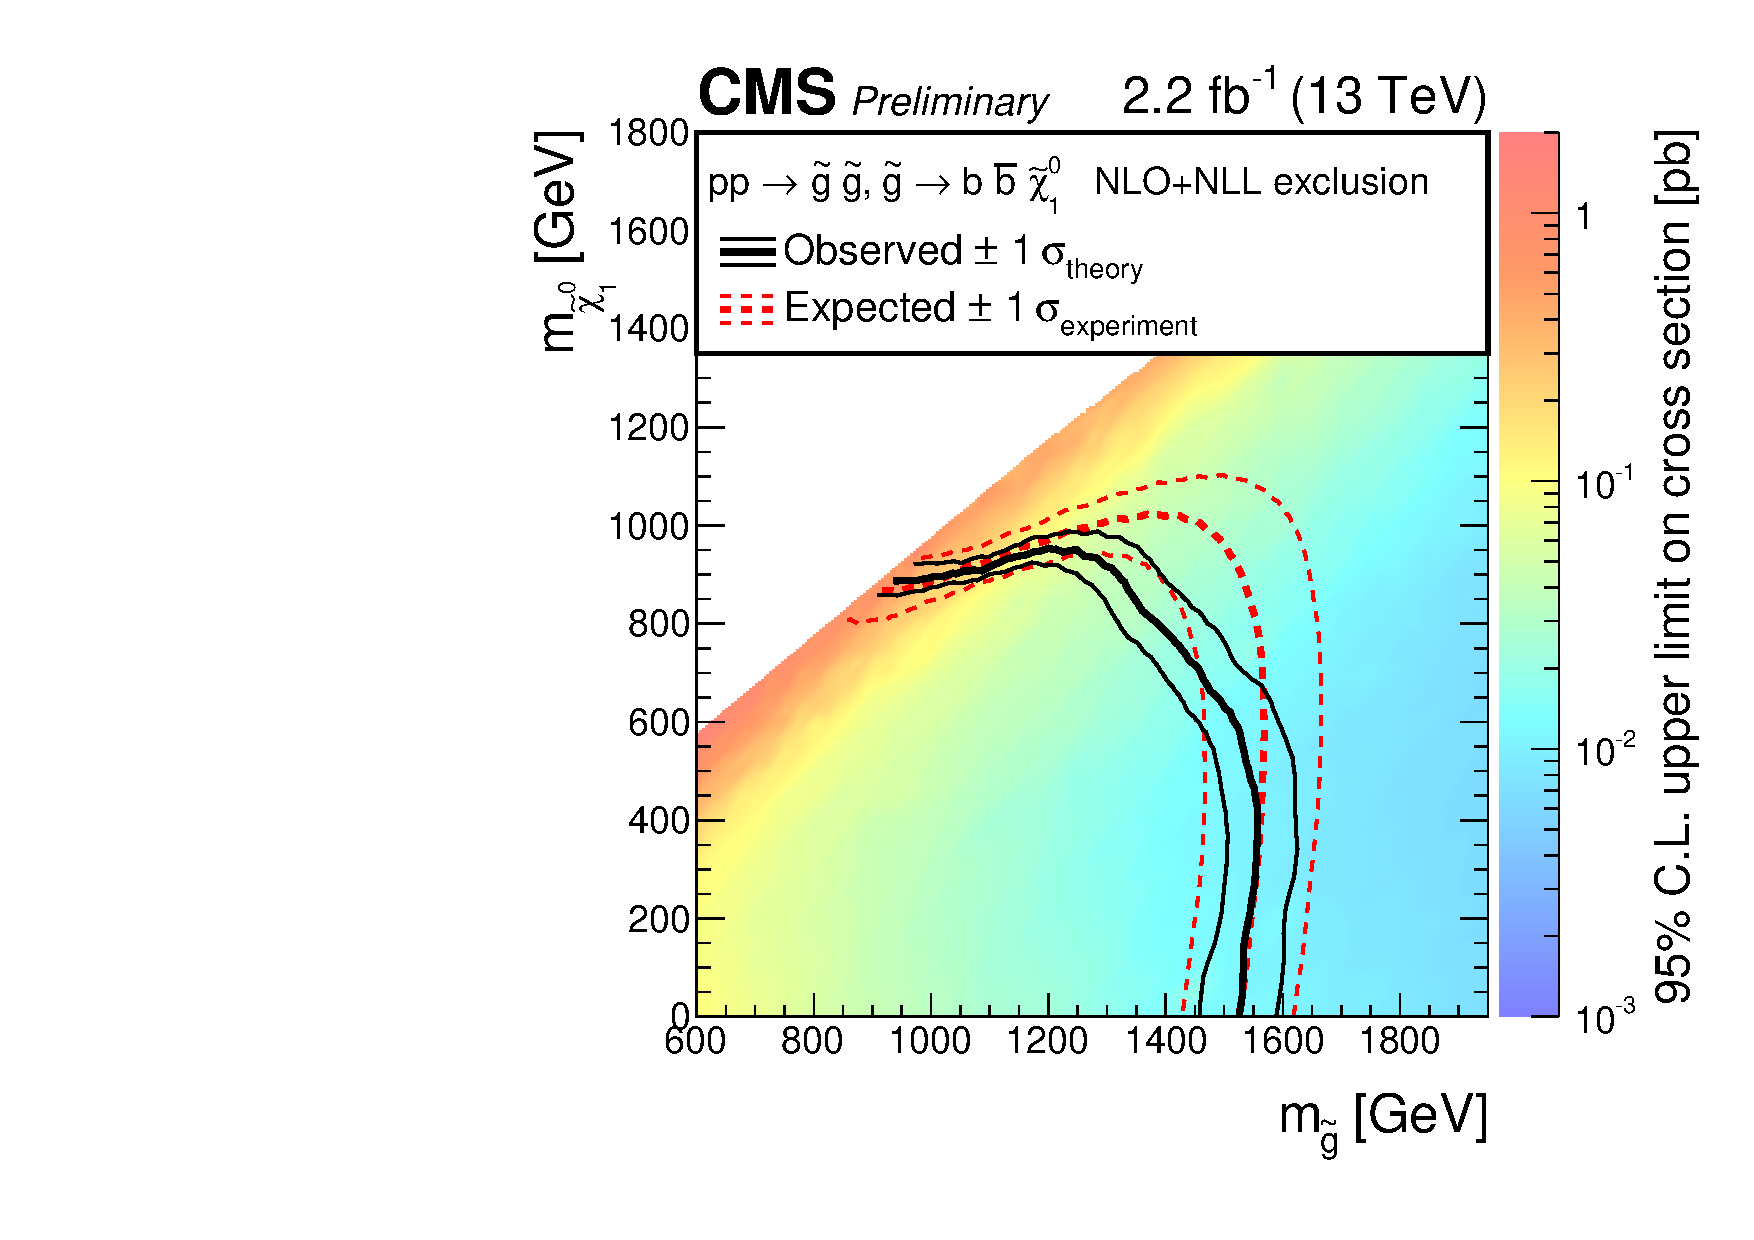
\includegraphics[width=0.5\textwidth]{figures/susyResults/t1bbbbRA1XSEC}} ~~
    \subfigure[T1qqqq]{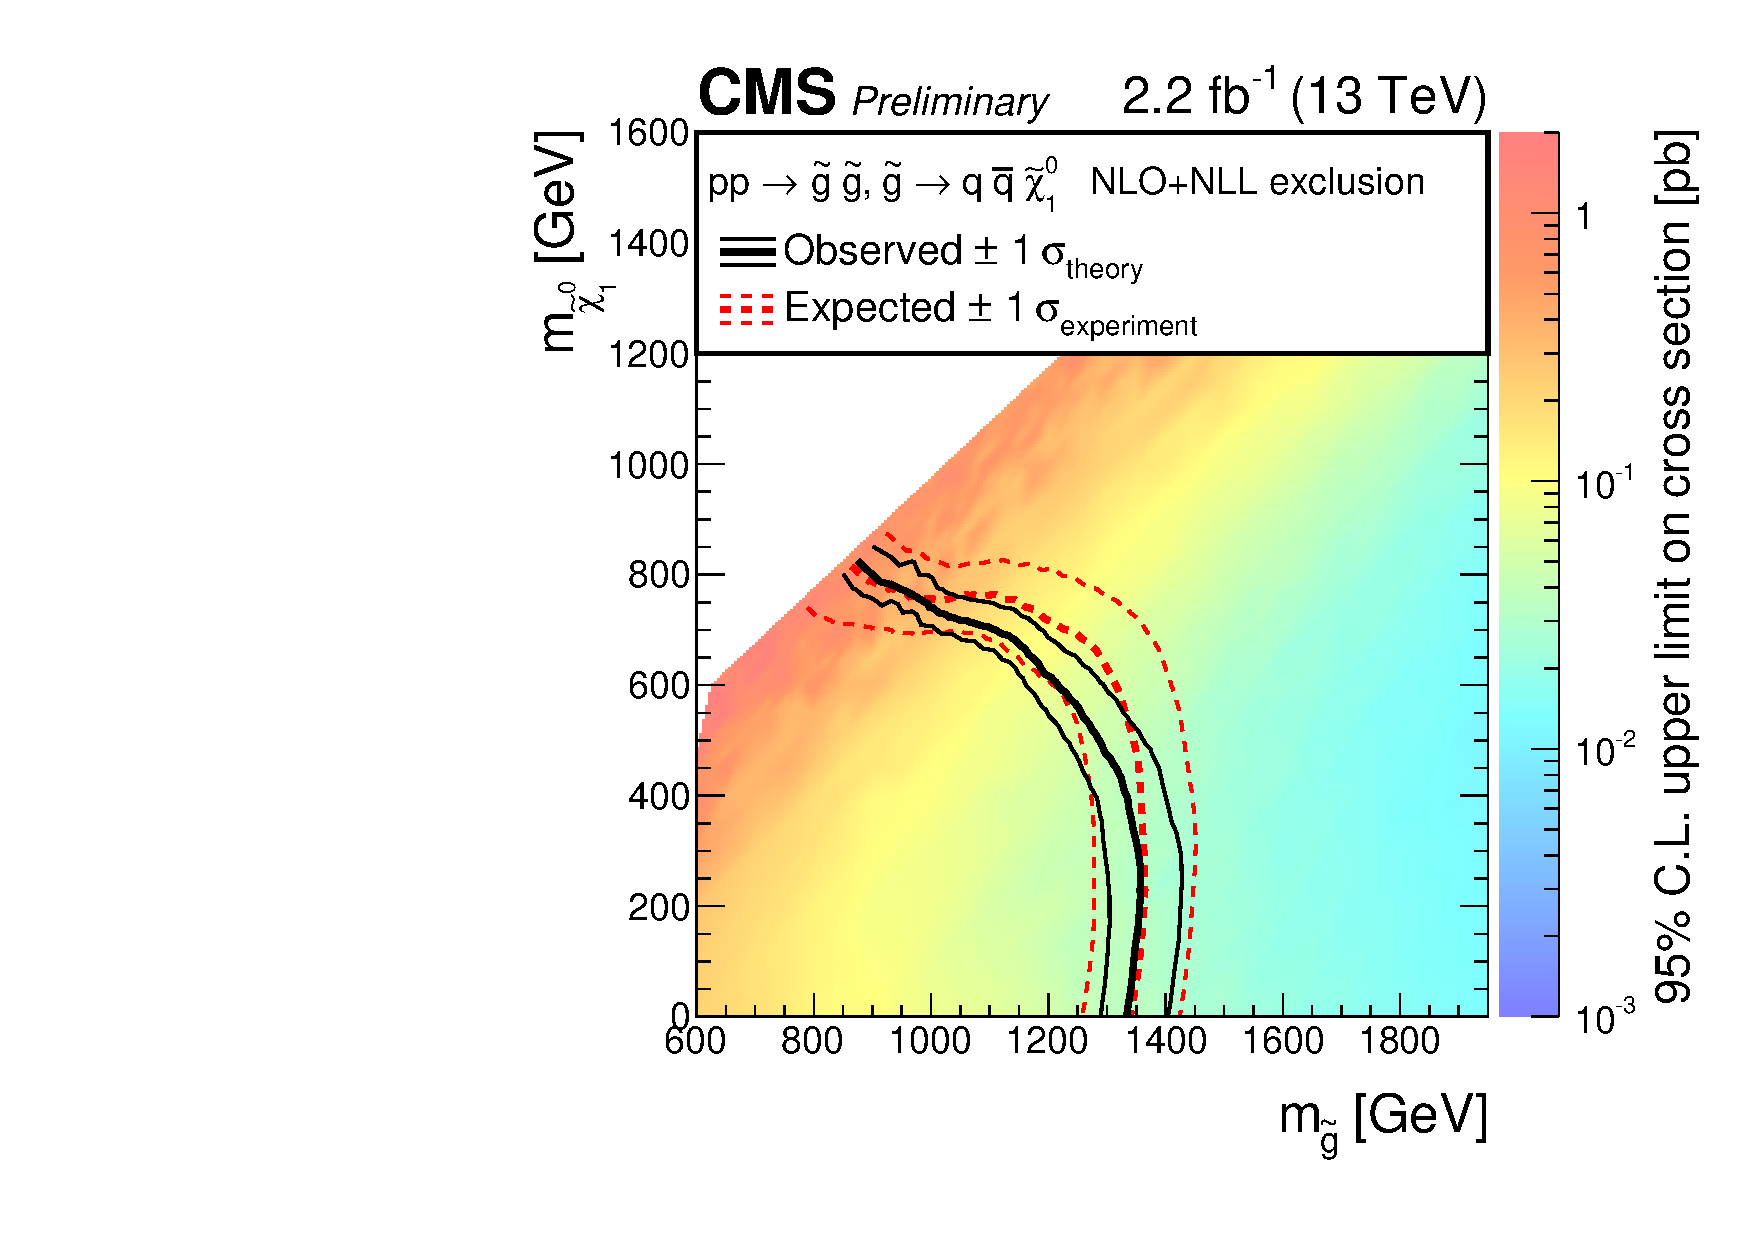
\includegraphics[width=0.5\textwidth]{figures/susyResults/t1qqqqRA1XSEC}} \\
    \subfigure[T1tttt]{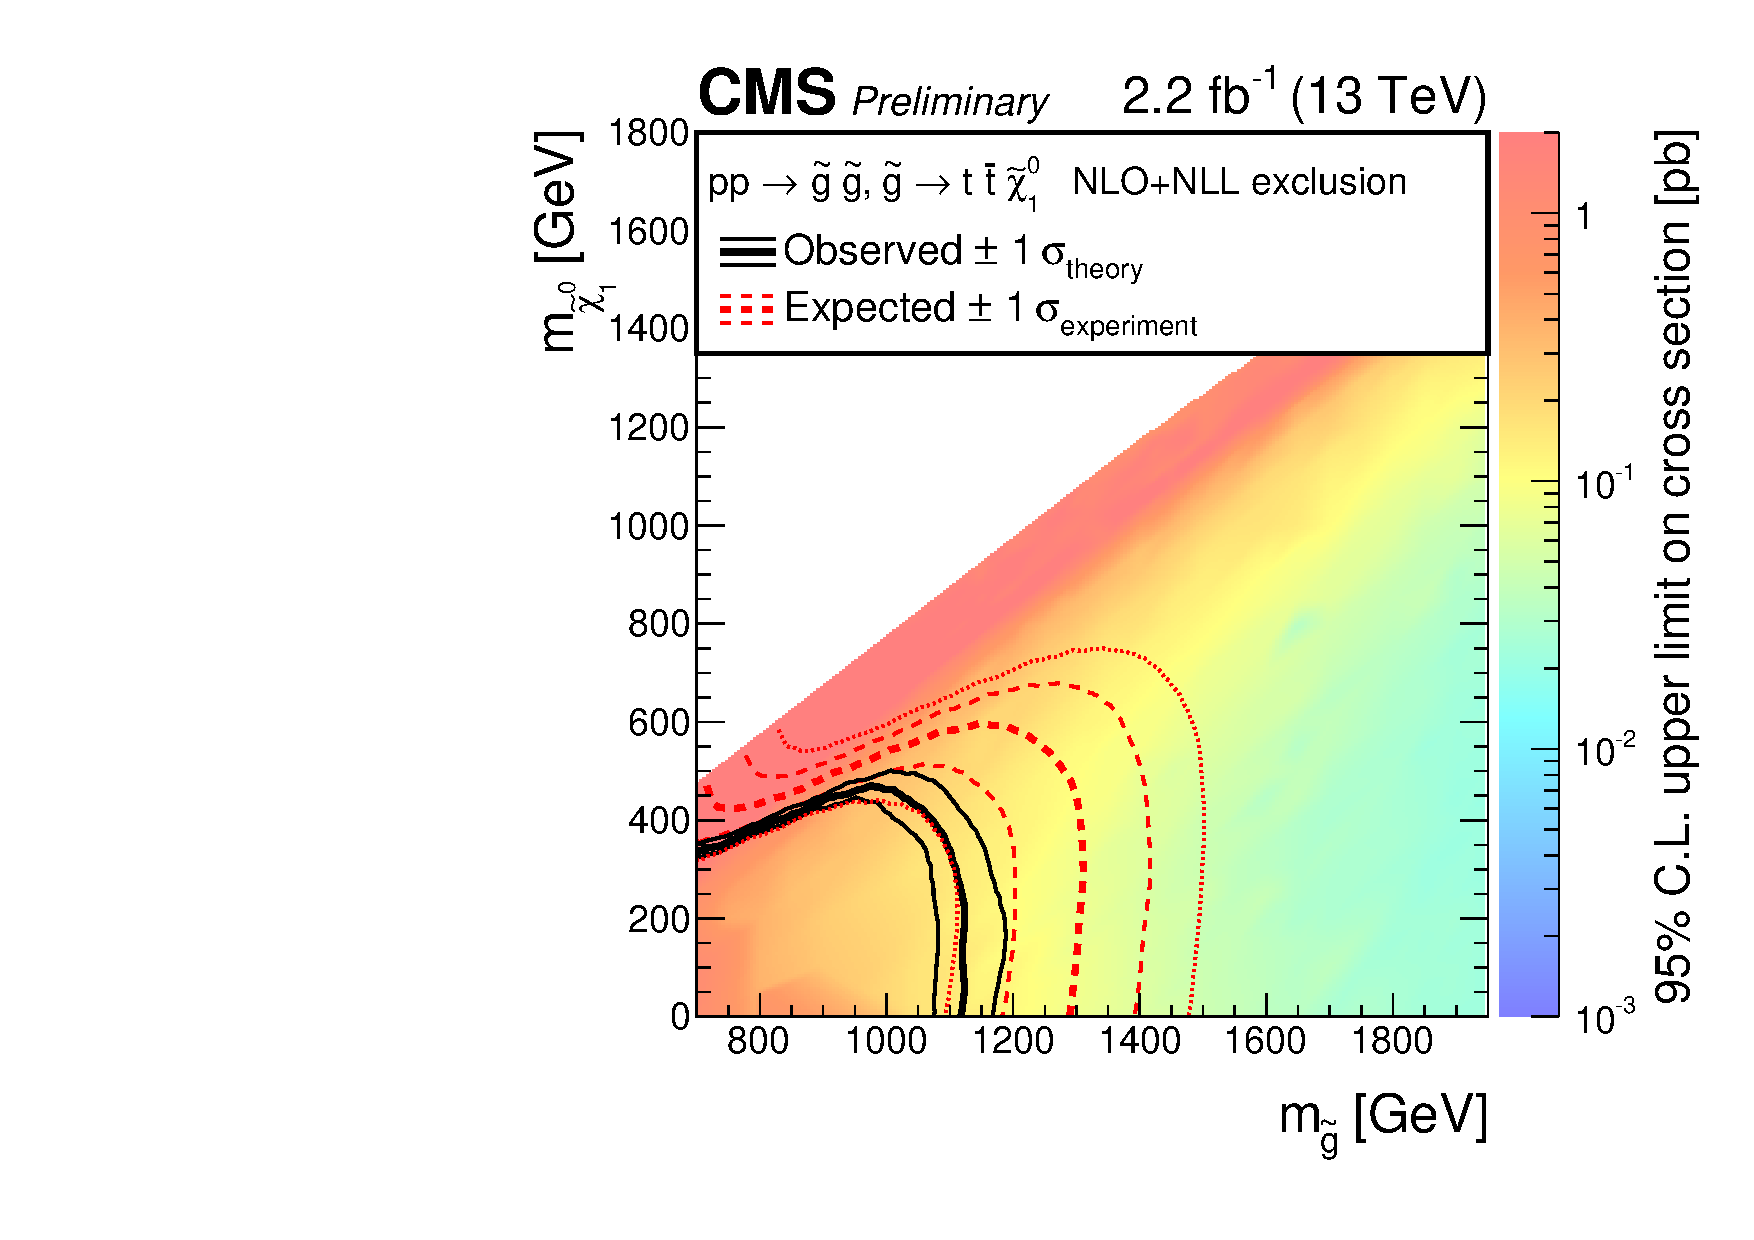
\includegraphics[width=0.5\textwidth]{figures/susyResults/t1ttttRA1XSEC}}
  \end{center}
\end{figure}





%%____________________________________________________________________________||
